\documentclass[a4paper, 12pt]{report}
\usepackage{monapack}
\usepackage{siunitx}
\usepackage{caption}
\usepackage{listings}
\usepackage{subcaption}
\usepackage{hyperref}
\usepackage{minted}
\usepackage[bottom]{footmisc}
\captionsetup[table]{skip=5pt}

%Proměnné
\student{Milan Jiříček}
\trida{B4.I}
\obor{18-20-M/01 Informační technologie}
\bydliste{Čenkov u Bechyně 3, 391--65 Bechyně}
\datumNarozeni{10. 11. 2001}
\vedouci{Ing. Břetislav Bakala}
\nazevPrace{Dálkové ovládání zásuvek NETIO}
\cisloPrace{12}
\skolniRok{2020/2021}
\reditel{Ing. Jiří Uhlík}

%Zadání
\begin{document}
    \nocite{*}
    \renewcommand{\listingscaption}{Úryvek kódu}


    \titulniStrana
    \section*{Anotace}
    Maturitní práce se zaměřuje na porovnání platforem ESP pro navrhovanou aplikaci.
    Cílem je vytvořit ovladač pro ovládání zásuvek značky NETIO s webovou aplikací pro konfiguraci a zjistit, která platforma je vhodná pro realizaci funkčního vzorku z hlediska spotřeby energie a~reakční doby.\\
    \textbf{Klíčová slova}\\
    ESP8266;\ ESP32;\ měření spotřeby;\ měření reakčního času;\ JSON;\ HTTP;\ NETIO;\ PowerCable

    \section*{Annotation}
    The graduation thesis focuses on the comparison of the ESP platforms for proposed application.
    The goal is to create a driver for controlling NETIO sockets with a web application for configuration and to find out which platform is suitable for the implementation of a~functional sample in terms of energy consumption and response time.\\
    \textbf{Keywords}\\
    ESP8266;\ ESP32;\ measuring usage;\ measuring time of reaction;\ JSON;\ HTTP;\ NETIO;\ PowerCable

    \podekovani
    Chtěl bych poděkovat panu učiteli Ing.~Břetislavu Bakalovi za odborné vedení práce a~cenné rady, které mi pomohly tuto práci zkompletovat.
    Rád bych také poděkoval technickému řediteli Ing.~Břetislavu Bakalovi ml.
    společnosti NETIO products a.s.\ za cenné rady, věcné připomínky a~vstřícnost při konzultacích a~vypracování maturitní práce.
    V~neposlední řadě chci poděkovat Mgr.~Haně Maříkové a~Mgr.~Vladimíře Špirhanzlové za~pomoc při gramatické a~stylistické kontrole.
    \tableofcontents


    \chapter{Úvod}\label{ch:uvod}
    %Teorie


    \chapter{Teoretický rozbor}\label{ch:teorie}


    \section{Netio PowerCable REST 101E}\label{sec:netio-powercable-rest-101e}
    PoweCable REST 101E, nebo také Cobra je chytrá zásuvka s možností WiFi připojení.
    Díky tomu je možné zásuvku ovládat přes řadu protokolů.
    Zásuvka také nabízí rozhraní otevřeného API, které umožňuje integraci do systémů třetích stran.
    Zásuvka také dokáže měřit napětí, el. proud nebo také např. příkon. \\
    K WiFi je možné se připojit přes uživatelské rozhraní.
    Pro moje účely využiji odesílání JSON dat pomocí HTTP\@.


    \section{Platforma ESP}\label{sec:platforma-esp}
    ESP jsou rodina mikročipů od společnosti \textbf{Espressif Systems}.

    \subsection{ESP8266}\label{subsec:esp8266}

    \subsubsection{Historie}
    \begin{figure}[h!]
        \centering
        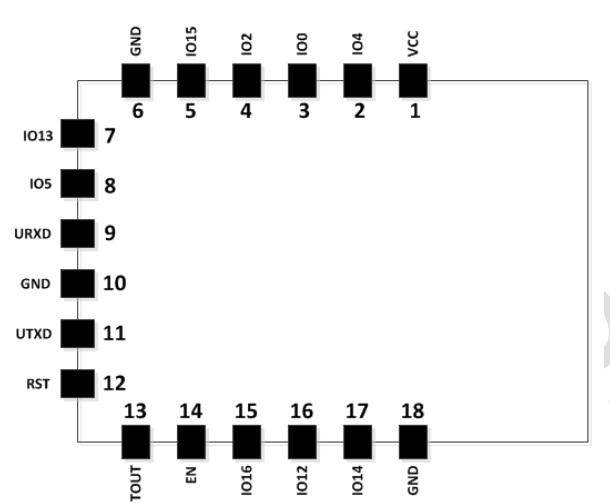
\includegraphics[width=9cm]{images/ESP8266_piny}
        \caption{ESP8266 pinout: literatura~\cite{WT8266}}
        \label{fig:esp8266_piny}
    \end{figure}
    ESP8266 je levný mikročip, který umí využívat WiFi. První chip, který se dostal na světlo světa byl v modulu \textbf{ESP-01}.
    Tento modul dokázal připojit se na WiFi síť a provádět jednoduché TCP/IP spojení. Získal si velkou oblibu díky nízké ceně.
    Jsou vhodné pro IoT jako například automatizace, zabezpečení, chytré domy atd.

    \subsubsection{Specifikace}
    Pro tuto maturitní práci bude použit modul \textbf{WT8266-S1}, který je vytvořen společností \textbf{Wireless-Tag}, protože tento modul je používán ve společnosti NETIO products a. s.\\
    ESP8266 integruje vylepšenou verzi procesoru \textbf{L106 Diamond series 32-bit} vytvořený firmou \textbf{Tensilica} s podporou frekvencí 80~\si{MHz} a 160~\si{MHz} a RTOS\footnote{Operační systém v realném čase}.
    K dispozici je RAM velká 36~\si{KB} a SPI flash paměť o velikosti 32~\si{Mb}.
    \begin{figure}[h!]
        \centering
        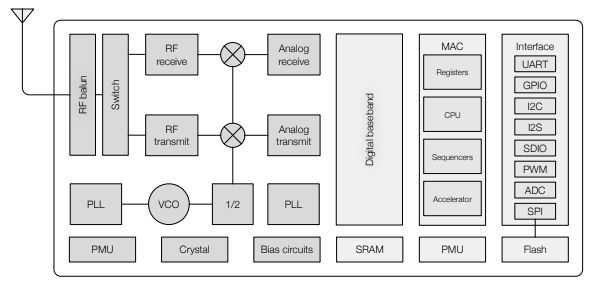
\includegraphics[width=11cm]{images/ESP8266_diagram}
        \caption{ESP8266 blokový diagram funkcí: literatura~\cite{ESP8266}}
        \label{fig:esp8266_diagram}
    \end{figure}

    Intergrovaný v systému je také 10 bitový analog-digitální převodník.
    Modul podporuje standard \textbf{IEEE802.11 b/g/n}\footnote{Standard pro lokální bezdrátové sítě} a sadu protokolů TCP/IP. WiFi 2,4~\si{GHz} umožňuje WPA/WPA2 \footnote{Chráněný přístup k WiFi}, rychlost až 72,2~\si{Mbps} a ke komunikaci využívá anténu PCB. Zařízení má 16~GPIO pinů\footnote{Vstupně výstupní pin} (\viz{fig:esp8266_piny}) z toho jsou některé piny využívány na specifické činnosti.
    Např. pokud při bootu ESP8266 přivedeme GROUND na GPIO~0, zařízení se přepne do UART\footnote{Univerzální asynchronní přijmač, vysílač} módu a je možné nahrát do flash paměti program. Další informace jsou na obrázku~\ref{fig:esp8266_diagram}.


    \subsection{ESP32}
    ESP32 je mladší model z řady ESP, který byl vydán v roce 2016.
    Tento mikročip má integrované WiFi i Bluetooth.
    Série ESP32 obsahuje mikroprocesor Tensilica Xtensa LX6 v dvou jádrové či jednojádrové verzi, který může operovat na 160~\si{MHz} nebo 240~\si{MHz}.
    RAM má velikost 520~\si{KB}.
    WiFi může dosáhnout rychlosti až 150~\si{Mbps} společně se zabezpečením WPA/WPA2. Kromě IPv4 je možnost použít i IPv6.
    ESP32 integruje 12 bitový analog-digitální převodník.
    Oproti ESP8266 je do tohoto modelu zabudován senzor teploty.
    ESP32 disponuje 36 GPIO piny.
    Další funkce jsou na obrázku~\ref{fig:esp32_diagram_pinout}. \\

    \begin{figure}[h!]
        \centering
        \begin{subfigure}[b]{0.4\linewidth}
            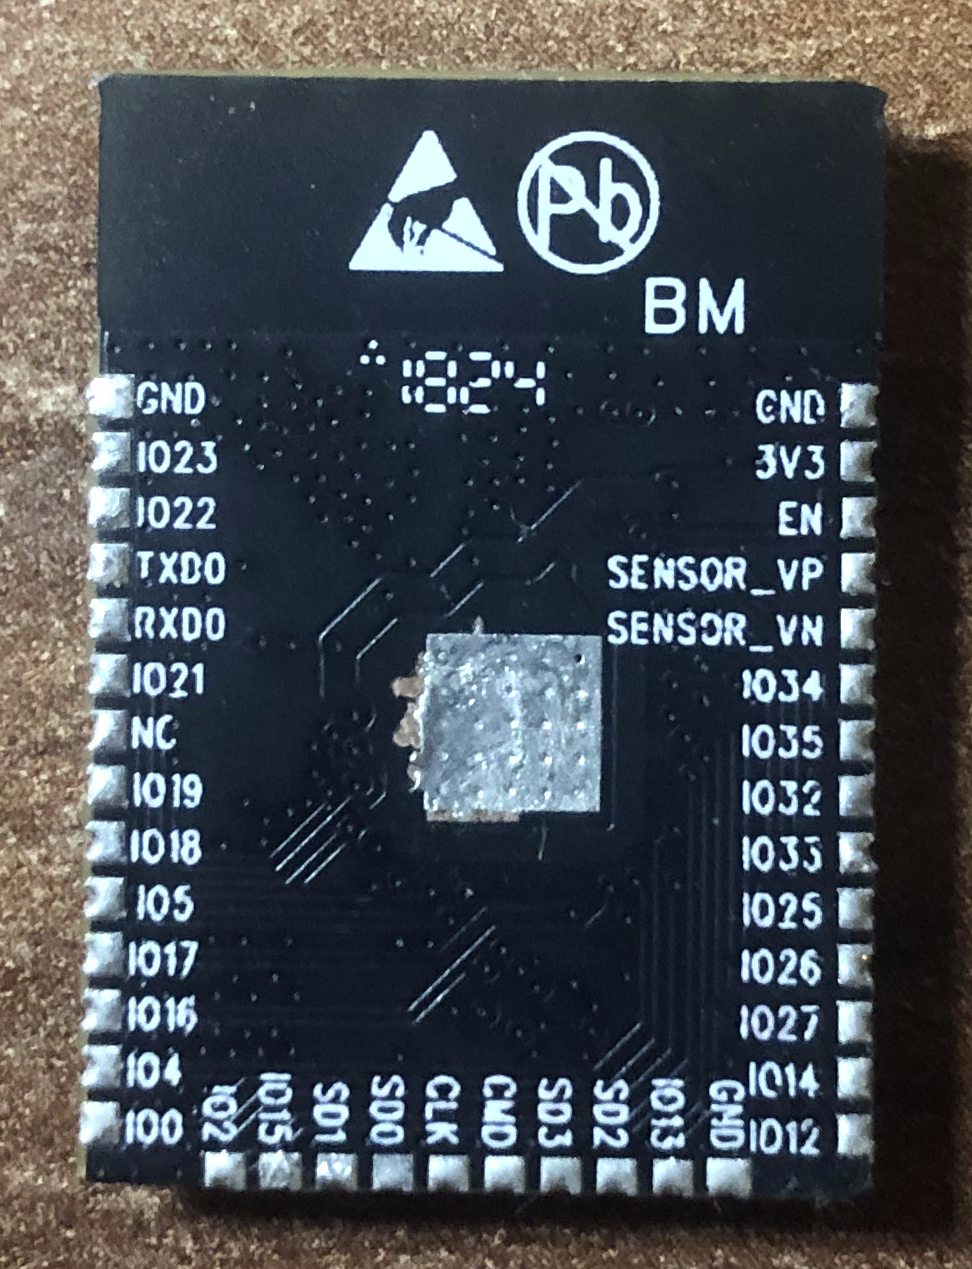
\includegraphics[width=\linewidth]{images/ESP32_piny}
            \caption{pinout}
        \end{subfigure}
        \begin{subfigure}[b]{0.5\linewidth}
            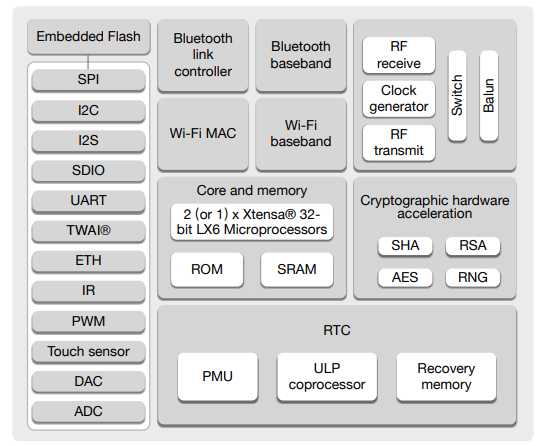
\includegraphics[width=\linewidth]{images/ESP32_diagram}
            \caption{blokový diagram: literatura~\cite{ESP32}}
        \end{subfigure}
        \caption{ESP32 pinout a blokový diagram}
        \label{fig:esp32_diagram_pinout}
    \end{figure}

    \subsection{Deep sleep} \label{subsec:deep-sleep}
    Platforma ESP lze také uvést do úsporného režimu.
    Jednoduše to znamená vypnutí nedůležitých částí po určitou doub.
    ESP8266 celkově nabízí 3 druhy úsporných režimů.
    Modem sleep, light sleep a deep sleep. \viz{fig:sleep_tabulka}.
    \begin{figure}[h!]
        \centering
        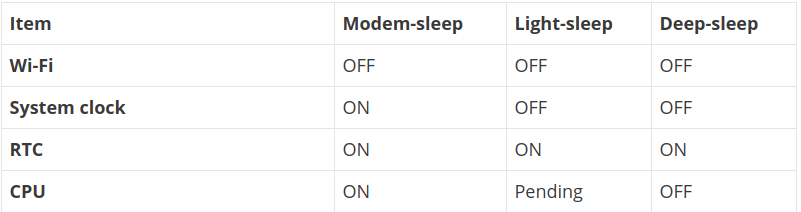
\includegraphics[width=11cm]{images/tabulka_sleep}
        \caption{podrobná tabulka sleep režimů: literatura~\cite{randomnerd}}
        \label{fig:sleep_tabulka}
    \end{figure}
    Pro moji maturitní práci použiji deep sleep, který poskytuje největší počet vypnutých částí včetně CPU či WiFi.
    Jedinou vyjimkou je \textbf{RTC}\footnote{Hodiny realného času}.
    V tomto režimu je také možné uchovat data v tzv. RTC paměti, která jsou dostupná i po obnovení.
    Průměrná spotřeba je 20 \si{\micro A} a je vhodný pro jakýkoliv projekt na akumulátor či baterii. \\
    Probuzení ESP8266 probíhá, buď po nastaveném čase, kde je nutné připojit pin \textbf{GPIO 16} tzv. wake-up pin na \textbf{RESET} (\viz{fig:esp8266_timed_pressed_deepsleep}a), ten po uplynutí nastaveného času se na krátkou dobu přepne z log. 1 na log. 0 a vyresetuje ESP8266, a nebo můžeme na \textbf{RESET}  přivést krátce tlačítkem logickou nulu a obnovíme ESP hardwarově (\viz{fig:esp8266_timed_pressed_deepsleep}b).
    \begin{figure}[h!]
        \centering
        \begin{subfigure}[b]{0.4\linewidth}
            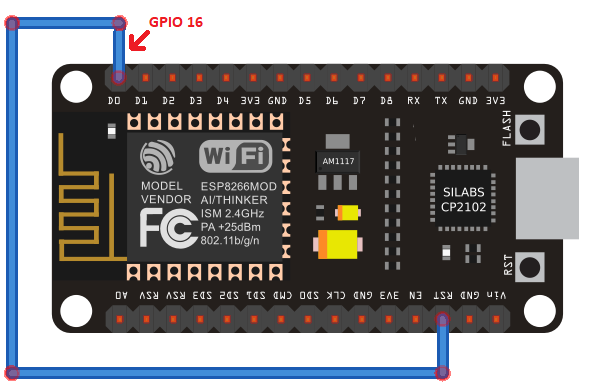
\includegraphics[width=\linewidth]{images/ESP8266_timed_deepsleep}
            \caption{Sotwarově po daném čase}
        \end{subfigure}
        \begin{subfigure}[b]{0.4\linewidth}
            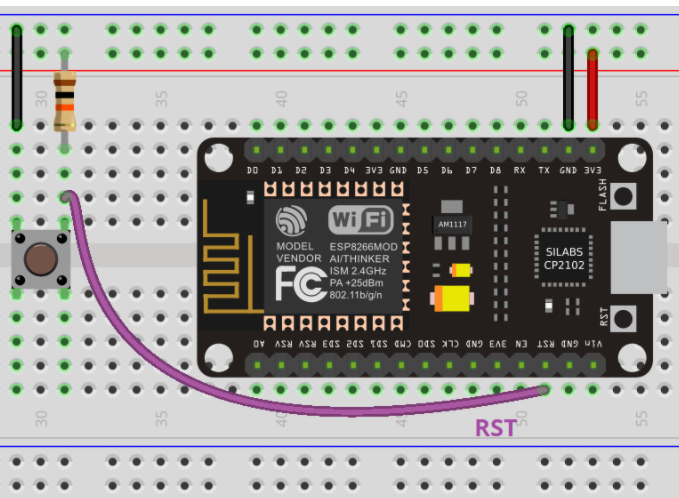
\includegraphics[width=\linewidth]{images/ESP8266_pressed_deepsleep}
            \caption{Hardwarově}
        \end{subfigure}
        \caption{ESP8266 probuzení z deep sleep po daném čase: literatura~\cite{randomnerd}}
        \label{fig:esp8266_timed_pressed_deepsleep}
    \end{figure}\\
    Jelikož ESP32 je novější model, deep sleep se liší v používání.
    ESP32 neprobouzíme přes RESET pin a proto se na mikročipu ani nenachází.
    Pokud chceme ESP probudit po určitém čase, nastavíme to pouze v programu a nemusíme žádné piny propojovat.
    V situaci hardwarového probuzení je nutné definovat pin probuzení a při jaké logické hodnotě se má probudit.
    Tento pin musí být tzv. RTC\_GPIO\footnote{Pin, který je v činnosti i během spánku ESP}.


    \section{LDLN030}
    LDLN030 je napěťový regulátor, který pracuje se vstupním napětím od 1,6 V do 5,5 V. Výstupní napětí dokáže stabilizovat na 3,3 V a pokud napětí klesne pod 3 V, odpojí zařízení napojené na výstupu.
    Klidový elektrický proud je 16 \si{\micro A} a logicky řízený enable pin uvede zařízení do vypnutého stavu, spotřeba elektrického proudu je nežší než 1 \si{\micro A}.
    Tato součástka má časté použití v mobilních telefonech, HDD a SSD discích, jelikož zařízení poskytuje nízký výstupní šum a vysoké PSRR\footnote{Schopnost obvodu udržovat výstupní napětí při změně vstupního napětí viz. literatura~\cite{PSRR}} \\
    Regulátor má celkem 5 pinů, a to vstup, výstup, GROUND, enable pin a Power Good.
    Enable pin rozhoduje zda součástka funguje či nikoliv, pokud je přivedena na zem, výstup je 0 V. Power Good je pin, který může informovat například základní desku během POST\footnote{Power On Self Test}, že napájení je v pořádku a může pokračovat v činnosti.
    %https://cs.wikipedia.org/wiki/Power_Good
    \begin{figure}[h]
        \centering
        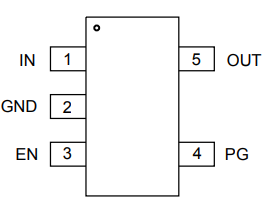
\includegraphics[width=9cm]{images/ldln030_datasheet}
        \caption{LDLN030 Pinout: literatura~\cite{stabilizator}}
        \label{fig:ldln030_datasheet}
    \end{figure}

    \begin{figure}[h]
        \centering
        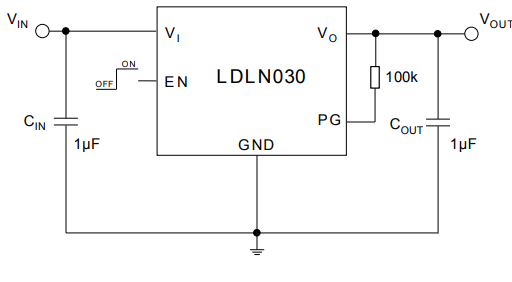
\includegraphics[width=9cm]{images/ldln030_datasheet2}
        \caption{LDLN030 Pinout: literatura~\cite{stabilizator}}
        \label{fig:ldln030_datasheet2}
    \end{figure}


    \section{Použité protokoly a jiné}

    \subsection{HTTP}
    HTTP je protokol pracující na aplikační vrstvě ISO/OSI modelu.
    Primárně je určen pro pro komunikaci s WWW servery a přenos hypertextových dokumentů ve formátu např. HTML\@.
    Typicky používá port TCP/80.
    Protokol funguje způsobem request/response\footnote{dotaz-odpověď}, kdy klient pošle request na požadovaný dokument.
    Server na to odpoví pomocí několika dat ohledně dotazu a poté požadovaným dokumentem.
    V mém projektu je použit pro žádání zásuvky o příslušnou akci.
    %https://en.wikipedia.org/wiki/Hypertext_Transfer_Protocol

    \subsection{JSON}
    JavaScript Object Notation je způsob zápisu dat nezávislých na platformě.
    Data mohou být organizována v polích nebo v objektech s jakýmkoliv datovým typem.
    JSON může složit k přenosu dat v libovolném programovacím či skriptovacím jazyku.
    Nevýhodou je, že nelze definovat znakovou sadu přenášeného obsahu, ale to platí jen pro některé implementace.
    V maturitní práci technologii JSON použiji jako nosič dat pro určení chování zásuvky a pro webserver.
    %https://cs.wikipedia.org/wiki/JavaScript_Object_Notation

    \subsection{DHCP}
    Dynamic Host Configuration Protocol je protokol z rodiny TCP/IP. Je určen pro automatickou konfiguraci zařízením připojených do dané sítě.
    DHCP server přiděluje zařízením IP adresu, masku sítě, defaultní bránu, adresu DNS serveru a čas, kdy jsou tyto údaje platné.
    Tato platnost se prodlužuje pokud je na zařízení zapnut DHCP klient.\\
    Klienti zažádají server o IP adresu tak, že klient po připojení do sítě vyšle broadcastem \textbf{DHCPDISCOVER} paket, na který odpoví DHCP server \textbf{DHCPOFFER} s nabídkou IP adresy.
    Klient si z nabídek vybere jednu IP adresu a o tu požádá paketem \textbf{DHCPREQUEST}.
    Server mu vzápětí potvrdí odpovědí \textbf{DHCPACK}, když klient obdrží tuto zprávu, může IP adresu používat.
    DHCP použiji pro připojení mého zařízení do bezdrátové sítě.
    %mirova otazka


    \chapter{Metodika postupu}


    \section{Tvorba měřecího vzorku}
    Pro měření jednotlivých scénářů jsem si vytvořil vzorek, který byl určen pouze na měření.
    Cílem bylo vytvořit vzorek jednoduše modifikovatelný, proto jsem zvolil pájivé pole na základní část.\\
    Na pájivém poli jsem napájel testovanou ESP platformu společně s přívodem, který byl 5 V. ESP má operační napětí 3,3 V, proto bylo nutné přidat stabilizator LDLN030, který napětí stabilizoval na operačním napětí.
    Stabilizátor byl zapojen dle doporučeného diagramu v datasheetu.
    Mezi zdrojem a IN pinem stabilizatoru jsem připojil bočník a vyvedl vodiče aby bylo možné měřit.
    \begin{figure}[h!]
        \centering
        \begin{subfigure}[b]{0.4\linewidth}
            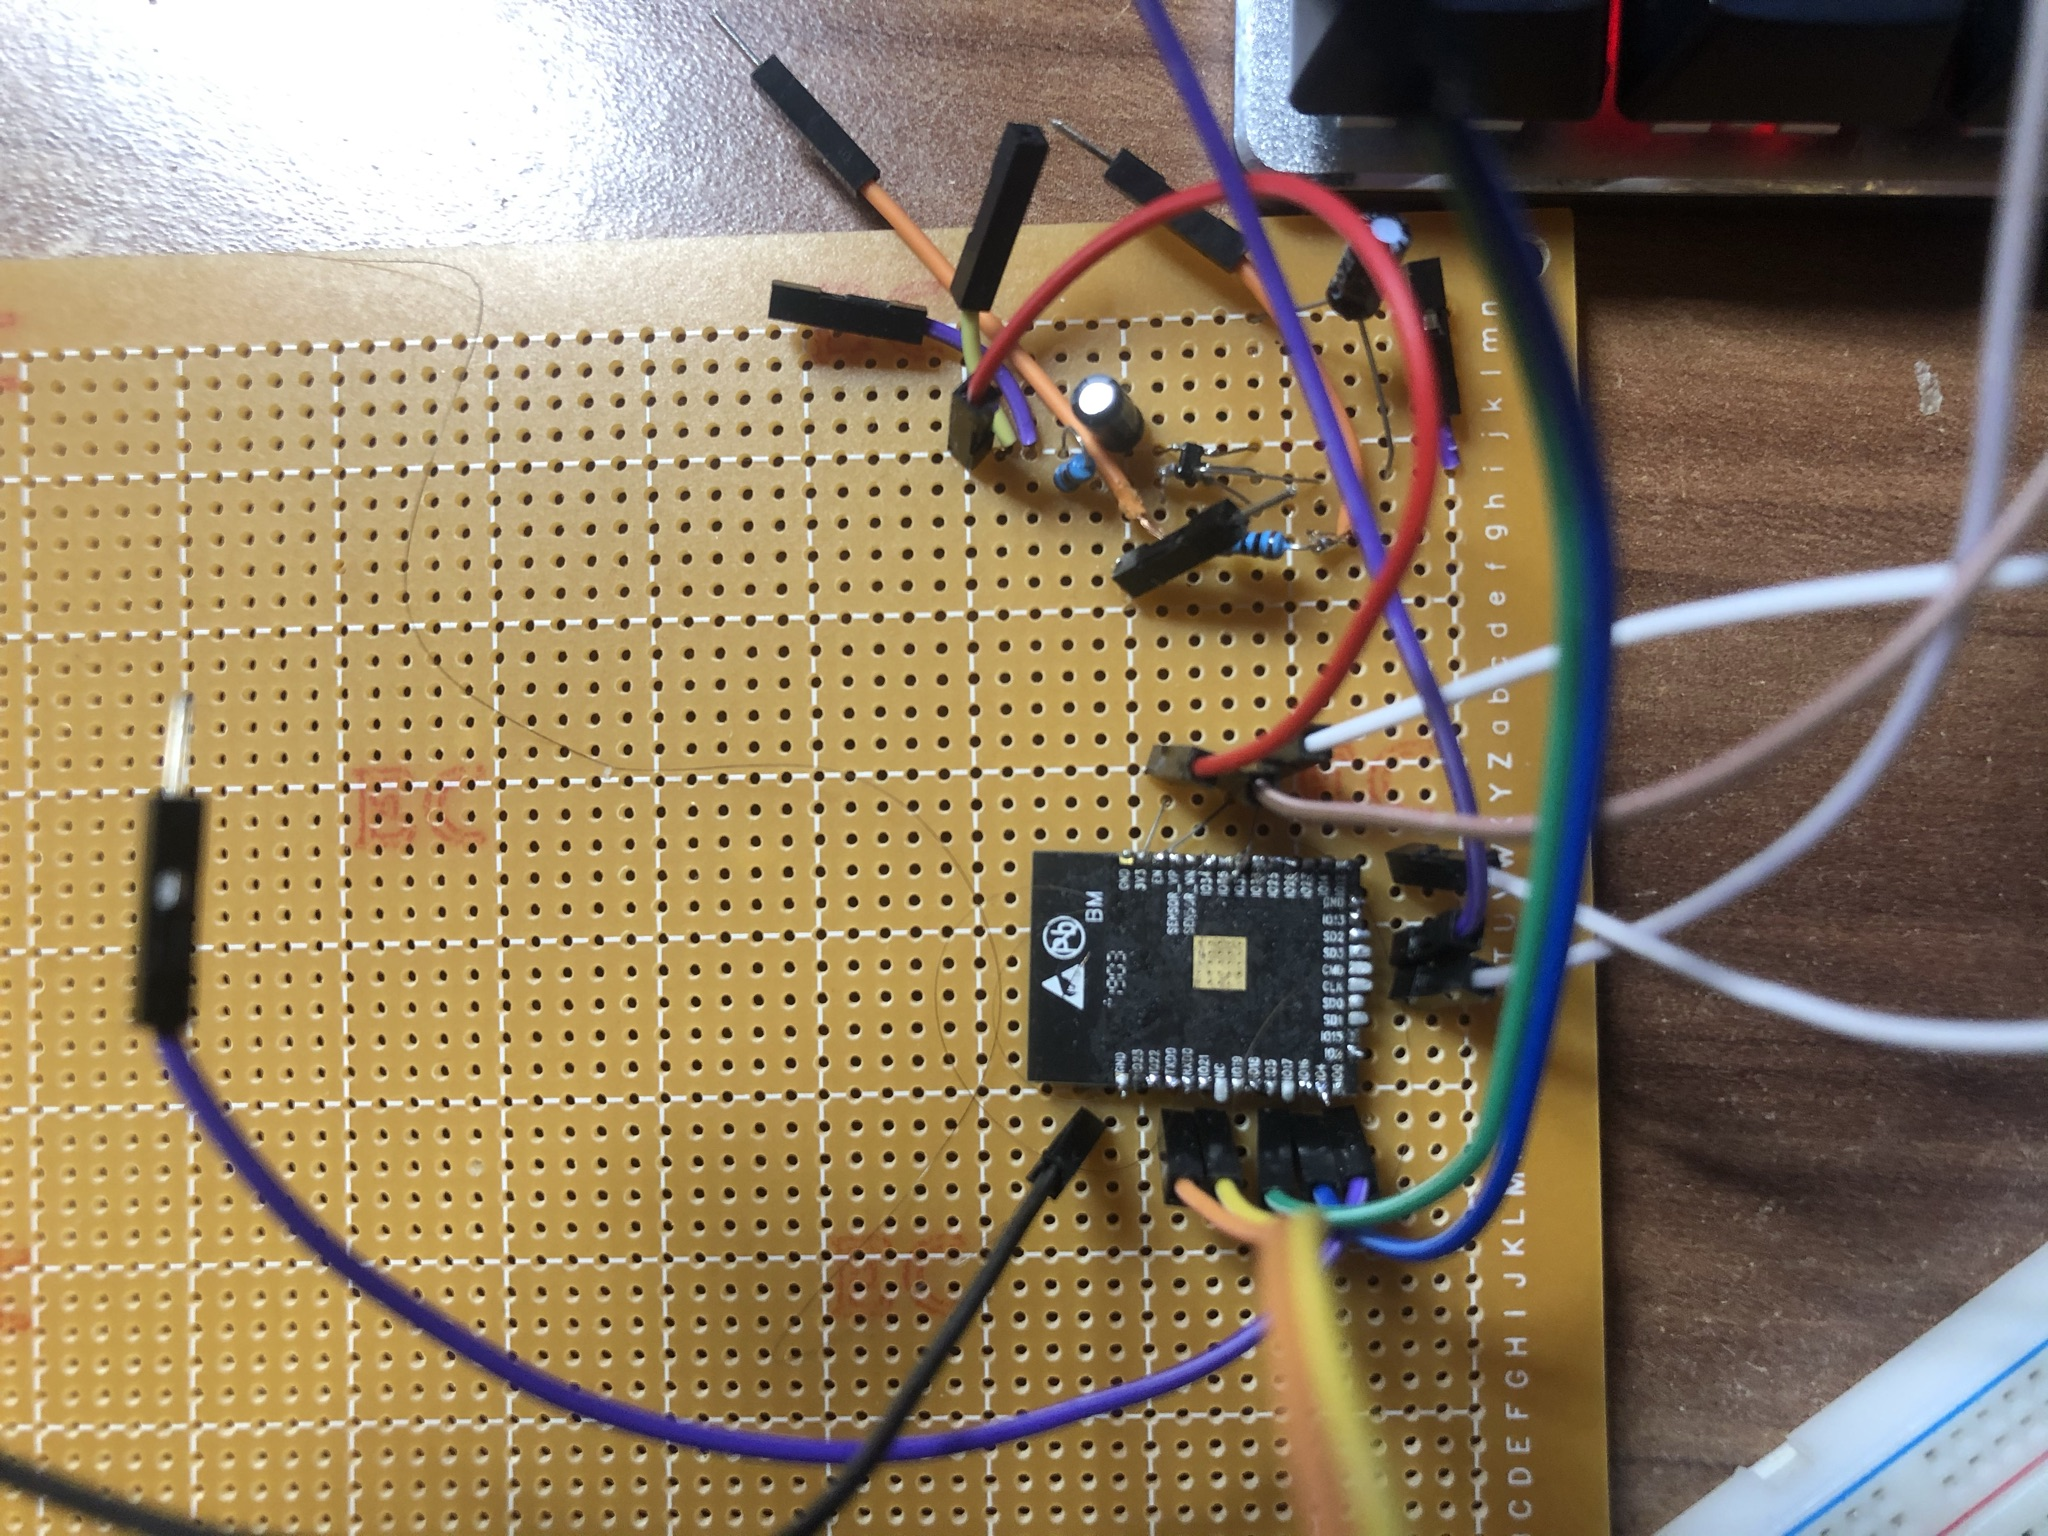
\includegraphics[width=\linewidth]{images/zapojeni_esp32_vzorek}
            \caption{Přední část}
        \end{subfigure}
        \begin{subfigure}[b]{0.4\linewidth}
            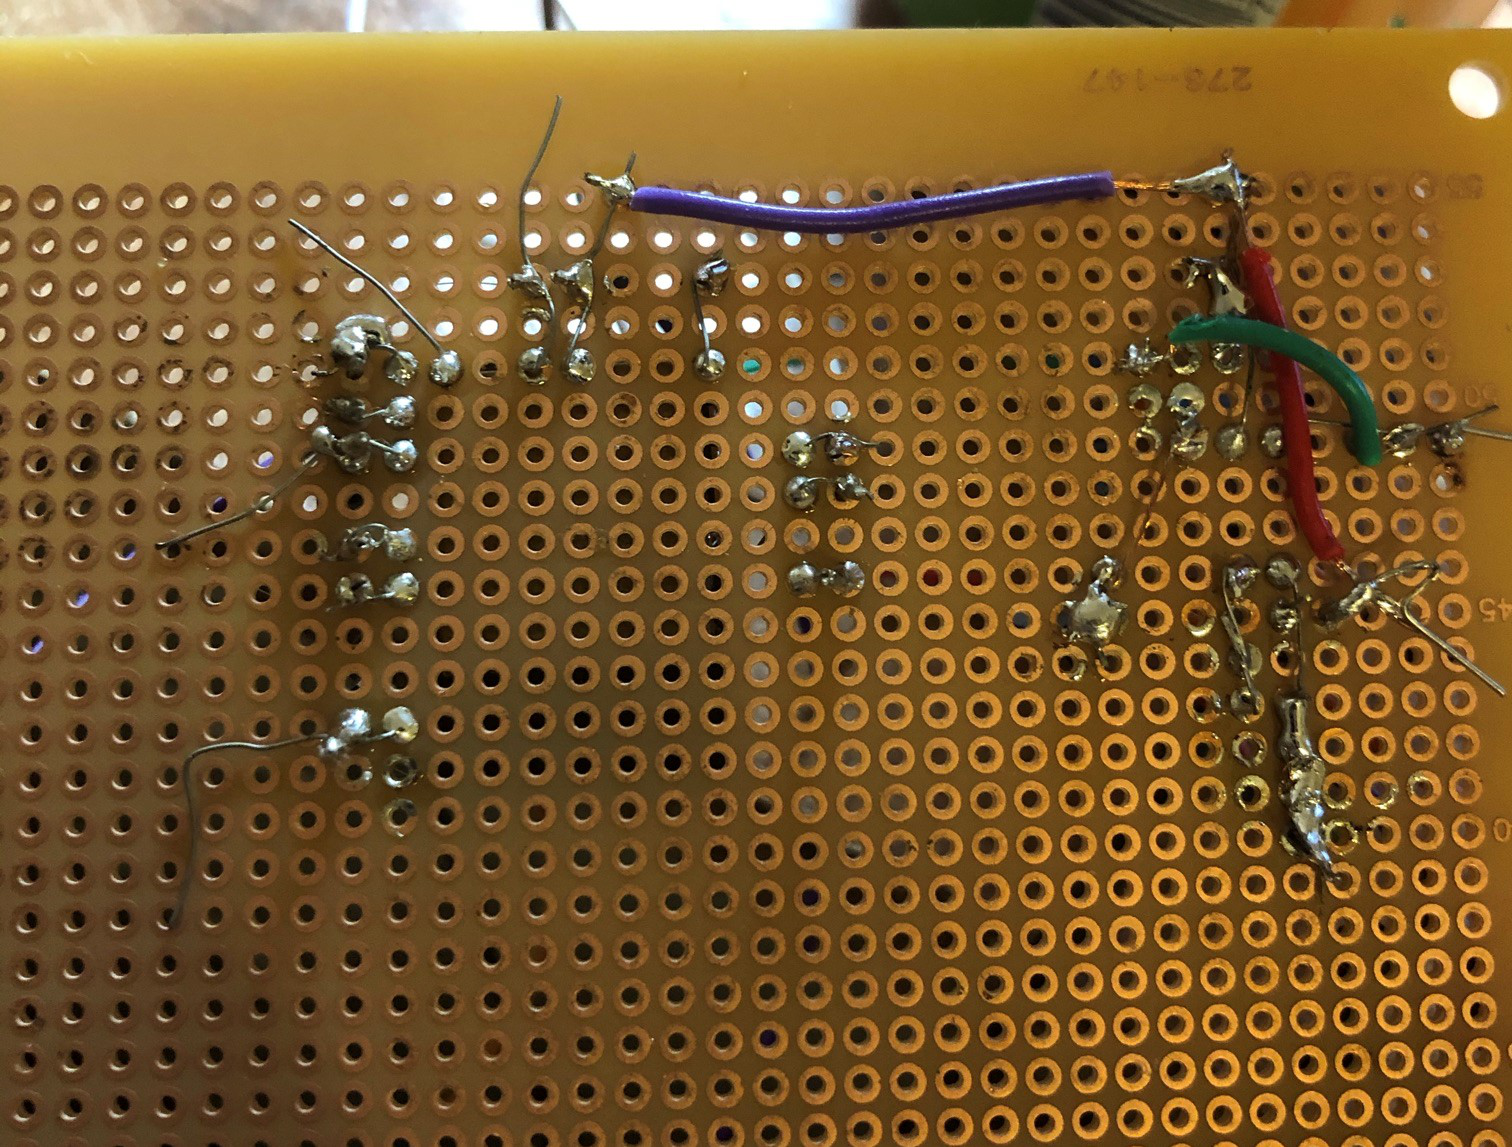
\includegraphics[width=\linewidth]{images/zapojeni_esp32_vzorek_zadek}
            \caption{Zadní část}
        \end{subfigure}
        \caption{Vzorek pro měření na pajivém poli}
        \label{fig:zapojeni_esp32_vzorek}
    \end{figure}\\
    Dále k potřebným GPIO pinům jsem napájel vodiče pro pozdější manipulaci.
    Pro další specifická zapojení, jako např. tlačítko, jsem použil nepájivé pole, které jsem vždy připojil specificky pro dané měření.\\


    \section{Měření připojení k WiFi a odeslání HTTP requestu}
    \label{sec:wifi}
    Cílem měření je zjistění rychlostí a spotřeby připojení různými způsoby k přístupovému bodu a~následné porovnání případů.
    Do měření je také započítáné odesílání HTTP requestu zásuvce.
    Jsou vytvořeny celkem 4 případy akcí:
    \begin{itemize}
        \item \textbf{statická IP adresa} - Zařízení dostane IP adresu, masku a bránu staticky nakonfigurovanou.
        Na access pointu bude vyplé DHCP a komunikace nebude zabezpečena.
        \item \textbf{dynamická IP adresa} - Bude využit DHCP protokol, kde zařízení požádá DHCP server o IP adresu, kterou mu access point přidělí společně s bránou, maskou a~s~časem, kdy tato adresa platí.
        Při měření nebude přístupový bod zabezpečen.
        \item \textbf{Zabezpečené připojení} - Připojení na access point bude šifrované pomocí WPA2~-~PSK. DHCP server bude zapnut.
        Toto je simulace klasického uživatelského používání.
        \item \textbf{Odeslání HTTP requestu} - Zařízení je připojené k WiFi. Odešle zprávu zásuvce a pokud dostane zpětnou vazbu od zásuvky, ukončí se činnost.
    \end{itemize}
    Ve všech scénářích bude měřeno zařízením \textbf{ANALOG DISCOVERY 2} od Digilent.
    Frekvence procesoru je 160 \si{MHz} a AP je vzdálen 3,5 \si{m} od zásuvky a funkčního vzorku ovladače.

    \subsection{Spotřeba}
    \label{subsec:wifi-spotreba}
    Měřen bude úbytek napětí na bočníku\footnote{nízkoohmový rezistor} o velikosti určené u měření.
    V programu k měřícímu zařízení je možné stejně jako na osciloskopu vytvořit graf naměřených hodnot v dané vzorkovací frekvenci.
    Hodnoty napětí bude převedeno na hodnoty el. proudu pomocí Ohmova zákona $I = \frac{U}{R}$.
    Amplitudy el. proudu budou sečteny a vyděleny počtem vzorků.
    Tato operace nám poskytne zjištění průměrného el. proudu ve scénáři.
    Spotřebu již vypočítáme dle:
    \[E = U \times \overline{I} \times \frac{t}{3600}\]
    Čas \textbf{t} v sekundách je možné zjistit v následující kapitole.

    \subsection{Reakční čas}
    \label{subsec:wifi-reakce}
    Z naměřeného případu bude vyjmuta klidová část a rozdíl mezi posledním a prvním vzorkem je poté reakční čas.
    V případě HTTP requestu nebude počítána část konfigurace WiFi.
    Společně s měřením byl na \textbf{serial monitor} odesílány zprávy, kde se program nachází.
    Poté se vyjmula část, která dle serial monitoru nepatří do scénáře.


    \section{Ustálené stavy}
    Pro ustálené stavy byly navrhnuty jednoduché programy pro co nejlepší porovnání.
    Ustálený stav je stav, kdy zařízení čeká na uživatelský podnět jako např. stisknutí tlačítka.
    Ideální ustálený stav musí splňovat:
    \begin{enumerate}
        \item nejkratší možnou reační dobu
        \item nejnižší možnou spotřebu pro co nejdelší výdrž baterií
    \end{enumerate}
    Reakční doba musí být v rámci uživatelské přívětivosti tzn. probuzení z tohoto stavu nesmí trvat více jak 1,5 \si{s}.
    Zároveň se zařízení nesmí vypnout zdůvodu vybité baterie za krátkou dobu. Porovnání proběhne mezi třemi scénáři, které mají jiné vlastnosti.
    Vybrány byly následující:
    \begin{itemize}
        \item \textbf{Kontinuální režim} - V tomto stavu není žádná funkce ESP vypnuta.
        \item \textbf{Deep sleep} - ESP vypne vše až na RTC (kapitola viz.~\ref{subsec:deep-sleep} na straně~\pageref{subsec:deep-sleep}).
        \item \textbf{Enable button} - ESP je vypnuto pomocí přivedené GROUND na pin ENABLE\@.
    \end{itemize}

    \subsection{Spotřeba}
    \label{subsec:ustalene-stavy-spotreba}
    Cílem měření je nalézt stav s nejmenší spotřebou energie, jelikož finální prvek bude napájen z baterií je důležité co nejdelší výdrž.
    Programy, které byly napsány pro měření:\\
    \begin{itemize}
        \item \textbf{Kontinuální režim} - Zařízení má nastavený určitý GPIO na tlačítko a monitoruje zda bylo zmáčknuto.
        ESP také má otevřenou sériovou komunikaci.
        \item \textbf{Deep sleep} - Program zajišťuje probuzení ESP každých 5 \si{s} a odesílání zprávy na serial monitoring.
        \item \textbf{Enable button} - Pro měření této situace není třeba specifický program
    \end{itemize}
    Pro měření bude použit \textbf{ANALOG DISCOVERY} s jeho funkcí osciloskopu.
    Na napájení bude přidán bočník o velikosti 0,7 \si{\ohm}, 10,5 \si{\ohm} nebo 4,7 \si{\ohm} \footnote{Je nutné zvolit takový odpor, aby byl úbytek napětí měřitelný.}.
    Pomocí Ohmova zákona $ I = \frac{U}{R} $ je možné zjistit el. proud.
    Příkon, který bude porovnán vypočítáme dle vztahu:
    \[P = U \times I\]

    \subsection{Probuzení z ustálených časů}
    \label{subsec:ustalene-stavy-reakce}
    Ovladač, který je již připojen k WiFi, po stisknutí tlačítka odešle HTTP request zásuvce, která zareaguje přepnutím stavu a odesláním zprávy zpět ovladači zda se povedlo či nikoliv.\\
    Reakční doba byla změřena pomocí kamery.
    K tlačítku jsem připojil LED, místnost jsem izoloval od světla a zmáčknutí tlačítka a reakci zásuvky jsem natočil ve zpomaleném režimu s \textbf{240 snímky za sekundu}.
    Pro upravení videa jsem použil trial verzi programu \textbf{Sony Vegas} (\viz{fig:sonyvegaspostup}).
    Našel jsem rozsvícení LED tlačítka a rozsvícení LED zásuvky ve videu a ustřihl jsem tento úsek od zbytku videa.
    Program poskytuje zobrazení počtu snímku daného úseku.
    Reakční čas je následovně možný zjistit pomocí:
    \[ t = \frac{\textrm{Počet snímků úseku}}{\textrm{Počet snímků za sekundu}}\]

    % MĚŘENÍ


    \chapter{Měření spotřeby a času}
    Všechny výpočty jsou k nalezení v adresáři Měření v souborech excel společně s použitými programy a naměřenými hodnotami v grafech.


    \section{ESP8266}

    \subsection{Spotřeba a reakční doba ustálených stavů}

    \subsubsection{Spotřeba}
    Spotřeba jednotlivých scénářů (\viz{fig:esp8266_waiting}) je měřena dle metodiky~\ref{subsec:ustalene-stavy-spotreba} na straně~\pageref{subsec:ustalene-stavy-spotreba}.
    Bočník pro měření úbytku napětí byl o velikosti 4,7 \si{\ohm}. \\
    Situace \textbf{enable button} nebyla možná změřit zařízením \textbf{ANALOG DISCOVERY 2} ani na bočníku o velikosti 0,7 \si{\ohm} kvůli velice nízkému úbytku napětí, který se v datasheetu WT8266 pohybuje v jednotkách \si{\micro A}.
    V tomto případě pro výpočty je použita hodnota, kterou určil výrobce v datasheetu.
    \begin{table}[h]
        \centering
        \caption{ESP8266 porovnání spotřeby ustálených stavů}
        \begin{tabular}{||l|r r r||}
            \hline
            Ustálený stav & U($V$) & I($A$)                  & P($W$)                 \\
            \hline
            Kontinuální   & $3,3$  & $67,66 \times 10^{-3}$  & $223,3 \times 10^{-3}$ \\
            Deep sleep    & $3,3$  & $138,20 \times 10^{-6}$ & $460,0 \times 10^{-6}$ \\
            Enable button & $3,3$  & $3,00\times 10^{-6}$    & $9,9\times 10^{-6}$    \\
            \hline
        \end{tabular}
        \label{tab:esp8266-klidove-rezimy-spotreba}
    \end{table}
    Dle tabulky~\ref{tab:esp8266-klidove-rezimy-spotreba} je možné vidět jednotlivé situace.
    Největším příkonem disponuje kontinuální ustálený stav z důvodu běžícího programu na kontrolu interakce.
    Nejmenší spotřeba je naopak vypnuté ESP přes enable pin. \\
    \begin{figure}[h!]
        \centering
        \begin{subfigure}[b]{0.6\linewidth}
            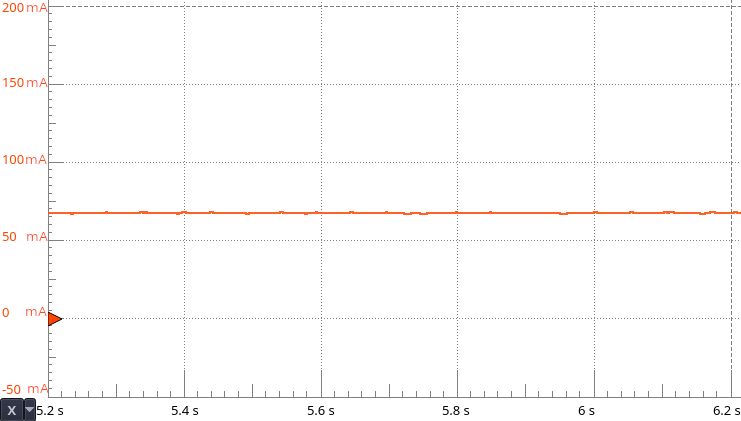
\includegraphics[width=\linewidth]{images/ESP8266_on_waiting}
            \caption{Kontinuální}
        \end{subfigure}
        \begin{subfigure}[b]{0.6\linewidth}
            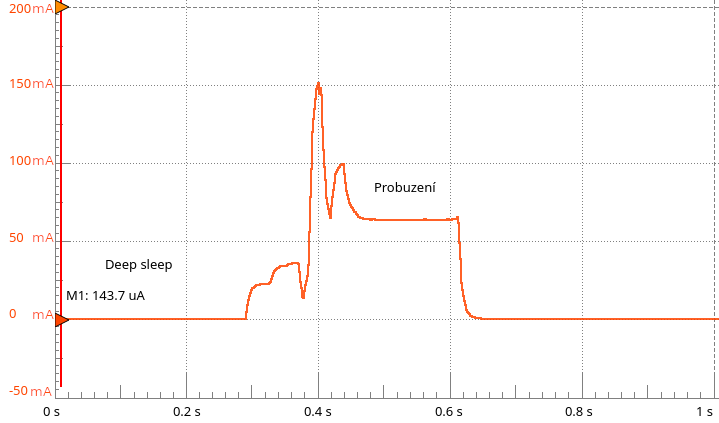
\includegraphics[width=\linewidth]{images/ESP8266_deepsleep_waiting}
            \caption{Deep Sleep}
        \end{subfigure}
        \caption{ESP8266 grafy ustálených režimů}
        \label{fig:esp8266_waiting}
    \end{figure}

    \subsubsection{Reakční čas}
    Reakční čas byl měřen dle metodiky~\ref{subsec:ustalene-stavy-reakce} na straně~\pageref{subsec:ustalene-stavy-reakce}.
    \begin{table}[]
        \centering
        \caption{ESP8266 porovnání reakčního času ustálených stavů}
        \begin{tabular}{||l|r||}
            \hline
            Ustálený stav & t(ms)          \\
            \hline
            Kontinuální   & \textbf{196}   \\
            Deep sleep    & \textbf{983}   \\
            Enable button & \textbf{3 208} \\
            \hline
        \end{tabular}
        \label{tab:esp8266-klidove-rezimy-cas}
    \end{table}
    Nejrychlejší ustálený stav je kontinuální, kvůli připravenosti na interakci \viztab{ESP8266 klidové režimy porovnani}.
    Nejdéle trvá vypnuté ESP, protože je nutné ESP zapnout, nastavit konfiguraci a připojit na WiFi, zatím co zapnuté ESP je již připraveno.

    \subsubsection{Porovnání}
    Pro porovnání spotřeb budeme předpokládat, že zařízení je napájeno 3$\times$ NiZn akumulátorem typu AA, které společně mají kapacitu \textbf{3750 mAh}, což je možné prevést na energii vztahem $E = U_{aku}\times \textrm{kapacita}$.
    a dále vztahem\footnote{$ t_{p}$ - provoz v ustáleném režimu, $ E_{bat}$ - energie 3$\times$ AA akumulátorů} $ t_{p} = \frac{E_{bat}}{P}$ zjistit provozní čas (\viztab{ESP8266 klidové režimy porovnani}).
    Zařízení není schopno dosáhnout této výdrže protože pokud napětí klesne pod 3 V, stabilizátor napájení odpojí.

    \begin{table}[h!]
        \centering
        \caption{ESP8266 porovnání ustálených stavů}
        \begin{tabular}{||l|r r r||}
            \hline
            Ustálený stav & P[$W$]                 & t$_{p}$[$h$]  & t[$ms$] \\
            \hline
            Kontinuální   & $223,3 \times 10^{-3}$ & $75,6$        & $196$   \\
            Deep sleep    & $460,0 \times 10^{-6}$ & $36 993,1$    & $983$   \\
            Enable button & $9,9\times 10^{-6}$    & $1 704 545,0$ & $3 208$ \\
            \hline
        \end{tabular}
        \label{tab:esp8266-klidove-rezimy-porovnani}
    \end{table}
    Kontinuální stav, zatímco má výdrž v rámci několika dní, reakční čas trvá necelých 200~ms.
    Enable button situace naprosto opačná.
    Reakční čas je pro uživatele dlouhý, ale výdrž v~tomto stavu bez interakce by se pohybovala v letech.
    Dobrý kompromis je situace deep sleep, kdy zařízení reagovalo vždy do jedné sekundy a teoretická výdrž je v jednotkách let.\\

    \subsection{Připojení k WiFi a odeslání HTTP requestu}
    Měření proběhlo dle metodiky~\ref{sec:wifi} na straně~\pageref{sec:wifi} na bočníku 0,7 \si{\ohm}.
    Z tabulky~\ref{tab:esp8266-spotreba-operaci} je možné vidět, že \textbf{příkon P} je téměř totožný v každé operaci.
    Největší rozdíl, který ovlivňuje spotřebu, je čas, za který se úkon vykoná.
    Jelikož \textbf{připojení pomocí statické IP adresy} trvalo nejkratší dobu, má také nejmenší spotřebu energie.
    Samotná \textbf{komunikace HTTP} má nejnižší spotřebu ze všech definovaných operací a jeden cyklus operace spotřebuje zanedbatelné množství energie.
    \newpage

    \begin{figure}[h!]
        \centering
        \begin{subfigure}[b]{0.65\linewidth}
            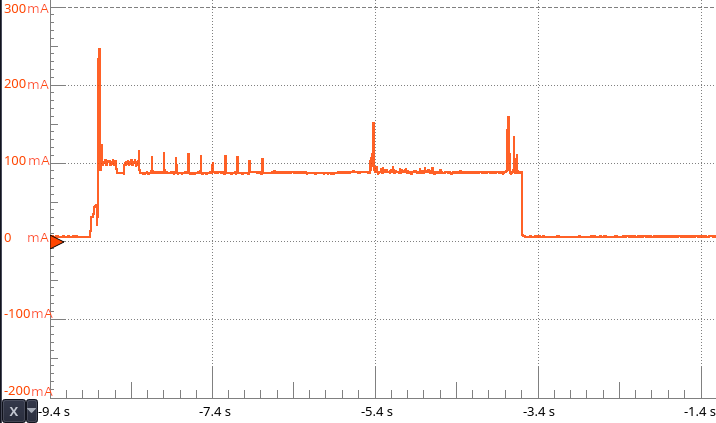
\includegraphics[width=\linewidth]{images/ESP8266_network_dynamic_specific}
            \caption{Dynamická IP}
        \end{subfigure}
        \begin{subfigure}[b]{0.65\linewidth}
            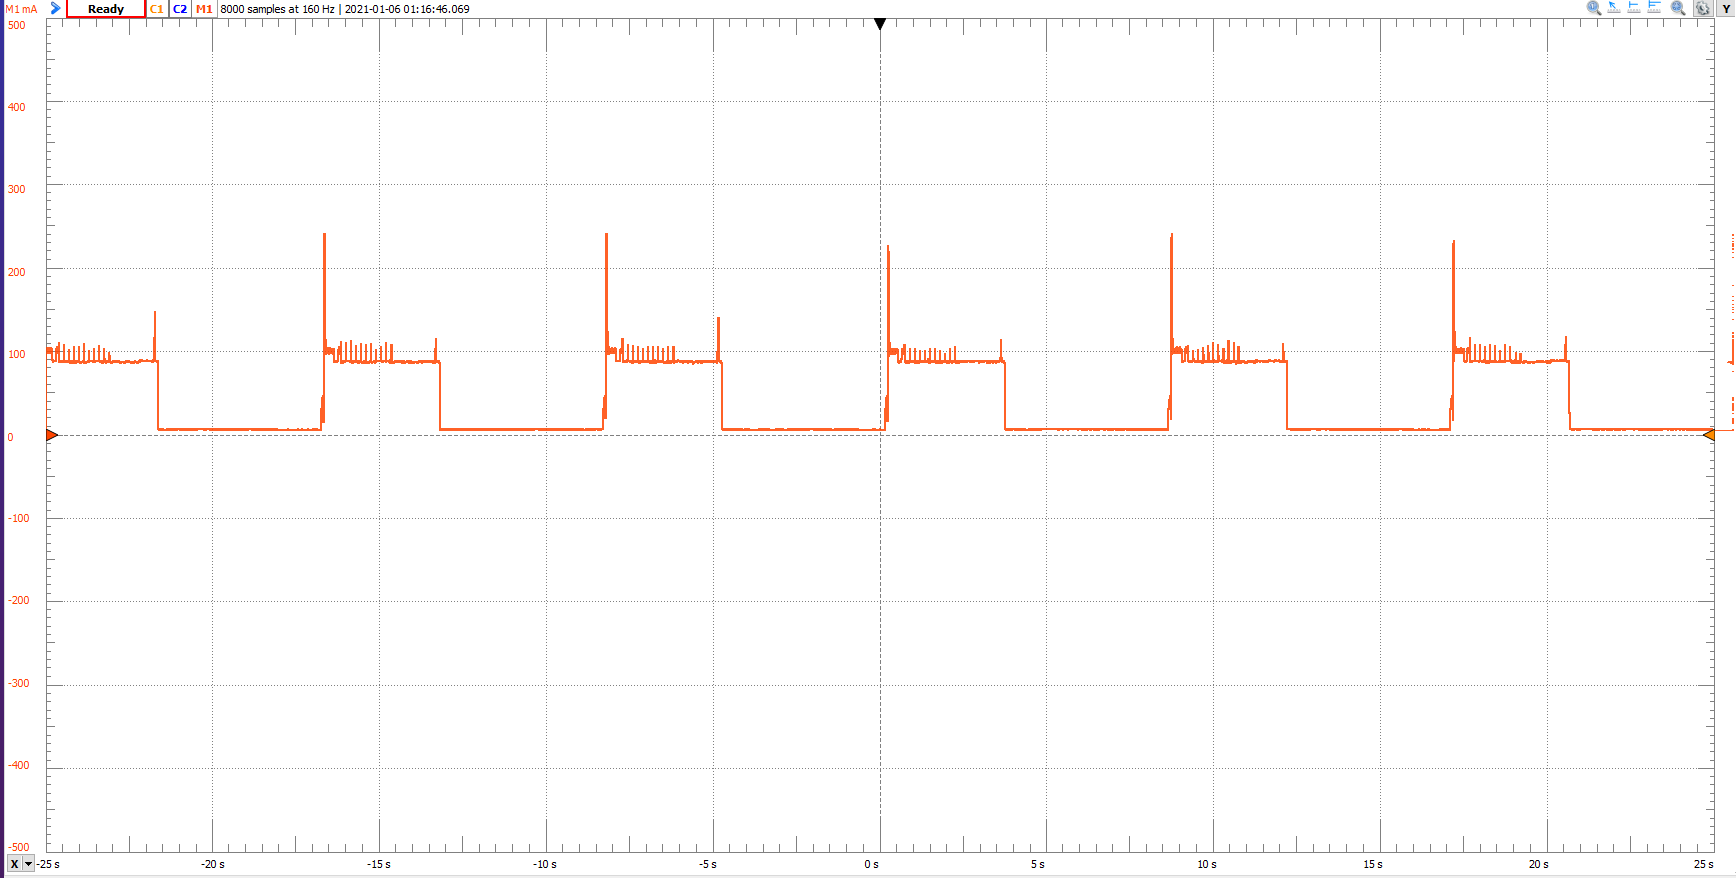
\includegraphics[width=\linewidth]{images/ESP8266_network_static}
            \caption{Statická IP}
        \end{subfigure}
        \begin{subfigure}[b]{0.65\linewidth}
            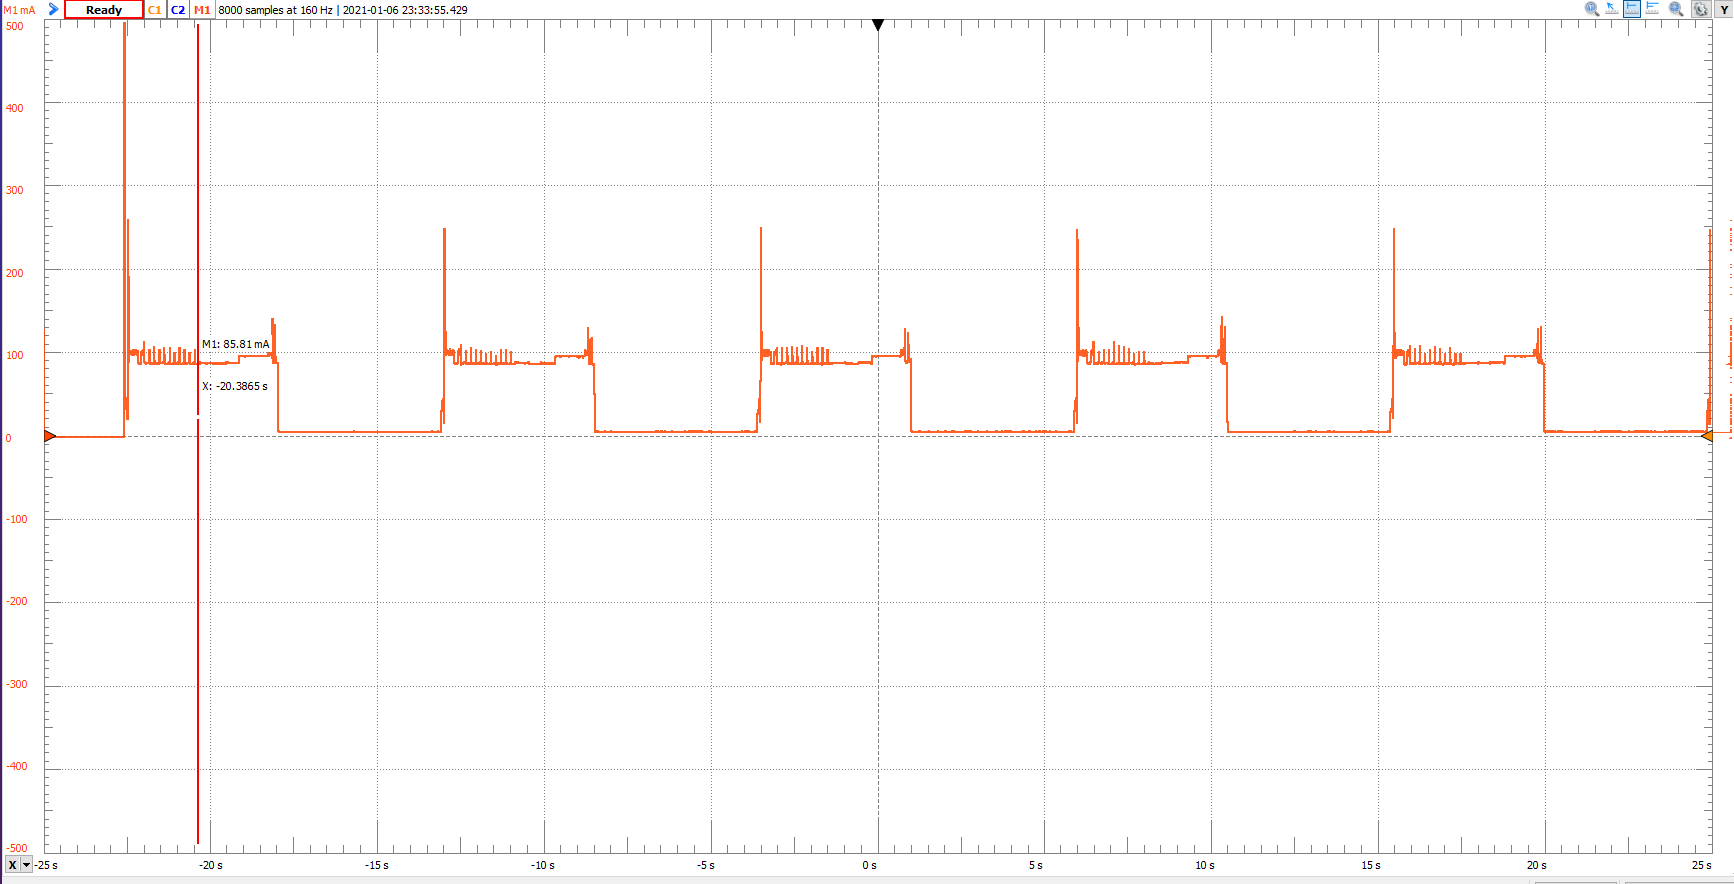
\includegraphics[width=\linewidth]{images/ESP8266_network_static_security}
            \caption{Zabezpečené, dynamická IP}
        \end{subfigure}
        \caption{ESP8266 grafy WiFi situací}
        \label{fig:esp8266_network}
    \end{figure}
    \newpage

    \begin{figure}[h]
        \centering
        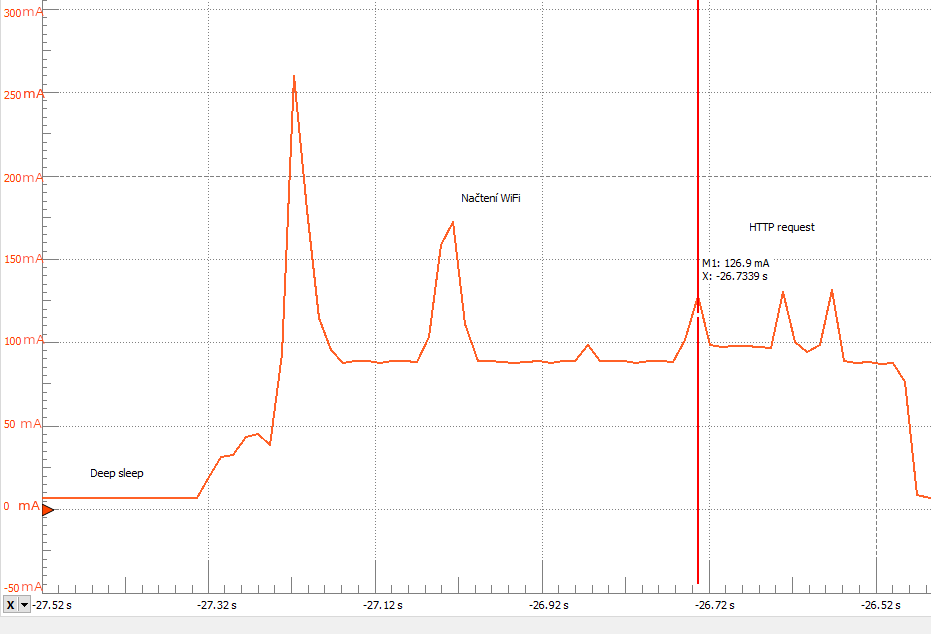
\includegraphics[width=12cm]{images/ESP8266_http}
        \caption{ESP8266 graf HTTP requestu}
        \label{fig:esp8266_http}
    \end{figure}


    \begin{table}[h]
        \centering
        \caption{ESP8266 Spotřeba operací}
        \begin{tabular}{||l| r r r r |r||}
            \hline
            Operace               & U(V) & I[$mA$] & t[$ms$] & P[$mW$] & \textbf{E}[$\mu Wh$] \\
            \hline
            \hline
            Dynamické připojení   & 3,3  & 89,5    & 5 300  & 295     & \textbf{435}         \\
            Statické připojení    & 3,3  & 83,0    & 3 143  & 274     & \textbf{239}         \\
            Zabezpečené připojení & 3,3  & 90,9    & 4 606  & 300     & \textbf{383}         \\
            HTTP komunikace       & 3,3  & 76,7    & 483     & 253     & \textbf{34}          \\
            \hline
        \end{tabular}
        \label{tab:esp8266-spotreba-operaci}
    \end{table}


    \section{ESP32}

    \subsection{Spotřeba a reakční doba ustálených stavů}

    \subsubsection{Spotřeba}
    Spotřeba jednotlivých scénářů je měřena dle metodiky~\ref{subsec:ustalene-stavy-spotreba} na straně~\pageref{subsec:ustalene-stavy-spotreba}.
    Bočník pro měření úbytku napětí byl o velikosti 10,5 \si{\ohm}.\\
    \begin{figure}[h!]
        \centering
        \begin{subfigure}[b]{0.6\linewidth}
            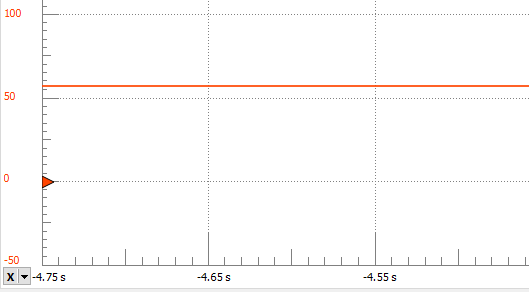
\includegraphics[width=\linewidth]{images/ESP32_on_waiting}
            \caption{Kontinuální}
        \end{subfigure}
        \begin{subfigure}[b]{0.6\linewidth}
            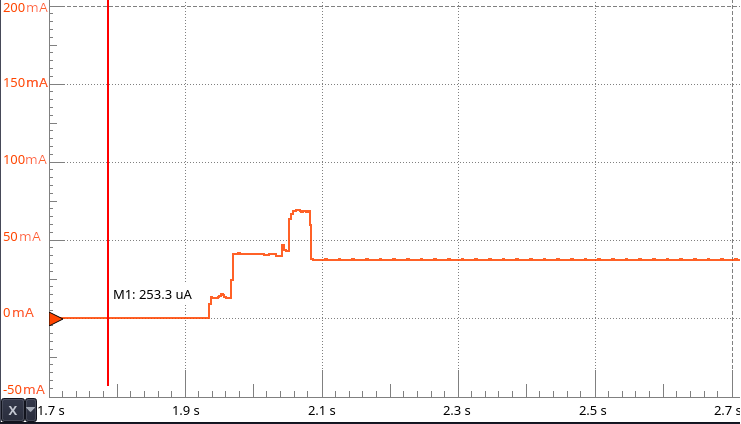
\includegraphics[width=\linewidth]{images/ESP32_deepsleep_waiting}
            \caption{Deep sleep}
        \end{subfigure}
        \caption{ESP32 grafy ustálených stavů}
        \label{fig:esp32-waiting}
    \end{figure}
    Ustálený stav enable pin nebyl naměřen zařízením Analog Discovery 2 z důvodu velmi nízkému úbytku napětí na bočníku.
    K porovnání bude použita hodnota z datasheetu.
    \begin{table}[h!]
        \centering
        \caption{ESP32 porovnání spotřeby ustálených stavů}
        \begin{tabular}{||l|r r r||}
            \hline
            Ustálený stav & U[$V$] & I[$A$]                  & P[$W$]                 \\
            \hline
            Kontinuální   & $3,3$  & $57,39 \times 10^{-3}$  & $189,4 \times 10^{-3}$ \\
            Deep sleep    & $3,3$  & $253,39 \times 10^{-6}$ & $838,0 \times 10^{-6}$ \\
            Enable button & $3,3$  & $1,00\times 10^{-6}$    & $3,3\times 10^{-6}$    \\
            \hline
        \end{tabular}
        \label{tab:esp32-klidove-rezimy-spotreba}
    \end{table}

    \subsubsection{Reakční čas}
    Získání reakčních časů jednotlivých možností zapojení ESP32 proběhlo způsobem dle~\ref{subsec:ustalene-stavy-spotreba} na straně~\pageref{subsec:ustalene-stavy-spotreba}.
    Tabulka~\ref{tab:esp32-klidove-rezimy-cas} ukazuje, že nejdéle trval ustálený režim v podobě vypnutého ESP32 přes enable pin a nejkratší dobu trval kontinuální ustálený stav.
    Kompromis mezi těmito dvěma stavy byl deep sleep ustálený stav, který se pohyboval okolo sekundy.

    \begin{table}[h]
        \centering
        \caption{ESP32 porovnání reakčního času jednotlivých situací}
        \begin{tabular}{||l|r||}
            \hline
            Ustálený stav & t[ms]           \\
            \hline
            Kontinuální   & \textbf{188}    \\
            Deep sleep    & \textbf{1 071} \\
            Enable button & \textbf{2 333} \\
            \hline
        \end{tabular}
        \label{tab:esp32-klidove-rezimy-cas}
    \end{table}

    \subsection{Připojení k WiFi a odeslání HTTP requestu}
    Měření proběhlo podle metodiky~\ref{sec:wifi} na straně~\pageref{sec:wifi}.
    \begin{table}[h]
        \centering
        \caption{ESP32 Spotřeba operací}
        \begin{tabular}{||l| r r r r |r||}
            \hline
            Operace               & U[V] & I[$mA$] & t[$ms$] & P[$mW$] & \textbf{E}[$\mu Wh$] \\
            \hline
            \hline
            Dynamické připojení   & 3,3  & 72,0    & 1406  & 238     & \textbf{92}          \\
            Statické připojení    & 3,3  & 69,2    & 1400  & 228     & \textbf{88}          \\
            Zabezpečené připojení & 3,3  & 74,7    & 1081  & 246     & \textbf{74}          \\
            HTTP komunikace       & 3,3  & 62,6    & 281   & 207     & \textbf{16}          \\
            \hline
        \end{tabular}
        \label{tab:esp32-spotreba-operaci}
    \end{table}
    \begin{figure}[h!]
        \centering
        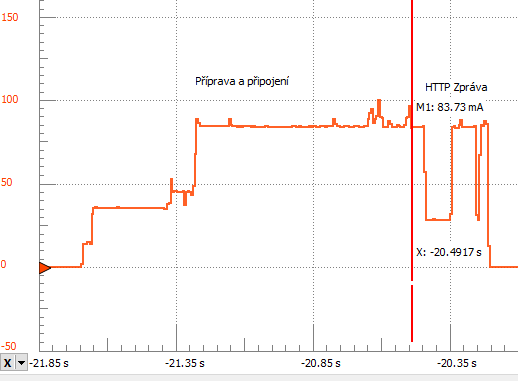
\includegraphics[width=12cm]{images/ESP32_http}
        \caption{ESP83 graf HTTP requestu}
        \label{fig:esp32_http}
    \end{figure}

    \begin{figure}[!ht]
    \centering
    \begin{subfigure}[b]{0.55\linewidth}
        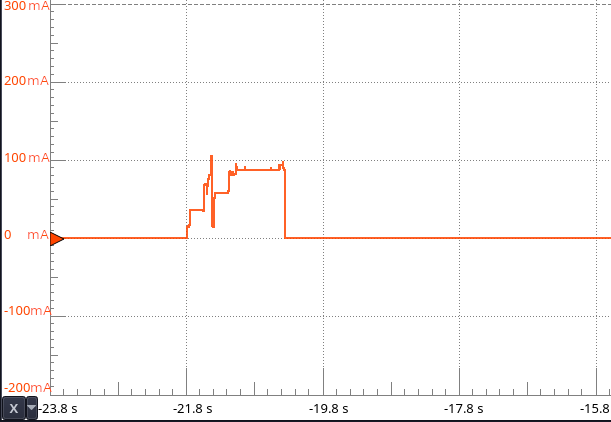
\includegraphics[width=\linewidth]{images/ESP32_network_dynamic}
        \caption{Dynamická IP}
    \end{subfigure}
    \begin{subfigure}[b]{0.55\linewidth}
        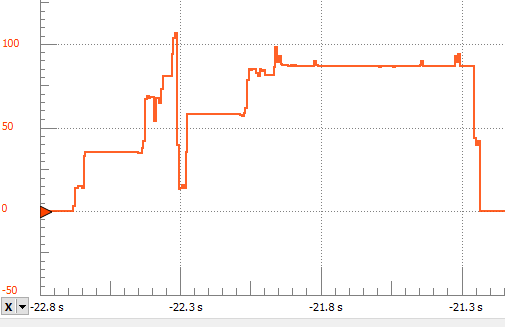
\includegraphics[width=\linewidth]{images/ESP32_network_static}
        \caption{Statická IP}
    \end{subfigure}
    \begin{subfigure}[b]{0.55\linewidth}
        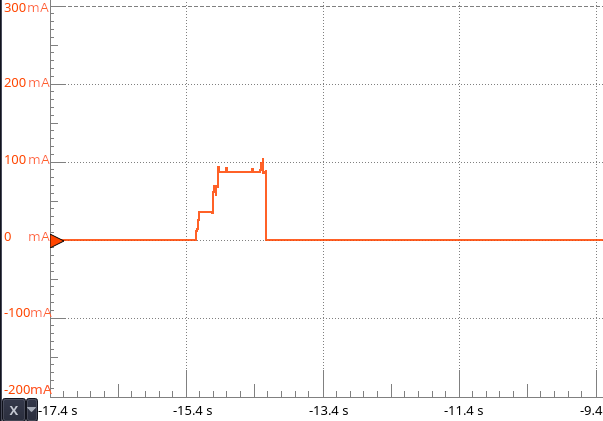
\includegraphics[width=\linewidth]{images/ESP32_network_static_security}
        \caption{Zabezpečené, dynamická IP}
    \end{subfigure}
    \caption{ESP32 grafy WiFi situací}
    \label{fig:esp32_network}
\end{figure}
    \newpage

    \section{Porovnání získaných výsledků}

    \subsection{Ustálené stavy}
    Z tabulky~\ref{tab:porovnani-klidove-rezimy-cas} je možné vidět jak si platformy vedly proti sobě. \\
    Pokud ovladač neustále běží s připojenou WiFi čas reakce je velmi rychlý a v obou případech uživatel nepostřehne prodlevu mezi aktivací ovladače a sepnutí relé v zásuvce.
    Časy mezi platformami se liší minimálně a rozdíl se pohybuje v rámci milisekund, přesto je ESP32 lehce rychlejší. \\
    Zapnutí vypnutého ESP, následné načtení a připojení k WiFi je nejdelší ze všech scénářů, který trvá několik sekund.
    Pro uživatele je velice pomalé a v realném produktu dle mého názoru zcela nepoužitelné.
    I přesto je ESP32 je mnohem rychlejší a to zhruba o 1 \si{s}.
    \begin{table}[h!]
        \centering
        \caption{Porovnání reakčních časů ústálených stavů platforem}
        \begin{tabular}{||l|r r||}
            \hline
            Ustálený stav & ESP8266        & ESP32          \\
            & [ms]           & [ms]           \\
            \hline
            Kontinuální   & \textbf{196}   & \textbf{188}   \\
            Enable        & \textbf{3 208} & \textbf{2 333} \\
            Deep sleep    & \textbf{983}   & \textbf{1 071} \\
            \hline
        \end{tabular}
        \label{tab:porovnani-klidove-rezimy-cas}
    \end{table}\\
    Deep sleep je alternativa mezi kontinuálním a vypnutým stavem.
    ESP totiž vypne vetšinu svých částí.
    Díky tomu je schopno relativně rychle zareagovat na budící signál.
    Reakce obou ovladačů cca 1 \si{s}.
    Zde vede ESP8266, které je zhruba o 100 \si{ms} rychlejší.
    Je to z důvodu komplikovanější struktury ESP32.
    Z tabulky~\ref{tab:porovnani-klidove-rezimy-spotreba} je možné porovnat elektrický proud a příkon jednotlivých ustálených stavů napříč platformami.
    Dle měření je kontinuální režim úspornější v ESP32.
    Větší rozdíl je možné nalézt během Deep sleep stavu.
    ESP8266 a ESP32 je liší skoro o dvojnásobek i přesto, že podmínky byly stejné.
    Stále se ale pohybujeme v řádech mikroWatt.
    Enable button stav kvůli citlivosti měřícího zařízení bylo možné porovnat pouze datasheet hodnoty.
    Zde je úspornější ESP32 ale stále jsou tyto hodnoty velice nízké.
    \begin{table}[h!]
        \centering
        \caption{Porovnání spotřeby ústálených stavů platforem}
        \begin{tabular}{||l|r r|r r||}
            \hline
            Ustálený stav & \multicolumn{2}{C|}{I[A]} & \multicolumn{2}{C||}{P[W]}   \\
                          & ESP8266        & ESP32   & ESP8266 & ESP32 \\
            \hline
            Kontinuální   & $67,66 \times 10^{-3}$   & $57,39 \times 10^{-3}$ & $233,3 \times 10^{-3}$& $189,4 \times 10^{-3}$ \\
            Deep sleep       & $138,20 \times 10^{-6}$ & $253,39 \times 10^{-6}$ & $460,0 \times 10^{-6}$&$838,0 \times 10^{-6}$\\
            Enable button    &  $3,00 \times 10^{-6}$   & $1,00 \times 10^{-6}$ & $9,9 \times 10^{-6}$&$3,3 \times 10^{-6}$\\
            \hline
        \end{tabular}
        \label{tab:porovnani-klidove-rezimy-spotreba}
    \end{table}\\
    Z hlediska poměru reakčního času a spotřeby je nejlepší ustálený stav deep sleep, jelikož reakční čas je přijatelný pro uživatele a díky nízkému příkonu zaření vydržet přijatelnou dobu.
    K sestavení funkčního vzorku proto bude použit tento ustálený stav pro obě platformy.
    \subsection{WiFi a HTTP}
    \begin{table}[h]
        \centering
        \caption{Porovnání operací}
        \begin{tabular}{||l| r r r r |r r||}
            \hline
            Operace & \multicolumn{2}{c}{t[ms]} & \multicolumn{2}{c}{P[mW]} & \multicolumn{2}{c||}{\textbf{E}[$\mu Wh$]} \\
            & ESP8266 & ESP32 & ESP8266 & ESP32 & ESP8266 & ESP32 \\
            \hline
            \hline
            Dynamické připojení   & 5300  & 1406    & 295  & 238     & \textbf{435}&\textbf{92}          \\
            Statické připojení    & 3143  & 1400    & 274  & 228     & \textbf{239}&\textbf{88}          \\
            Zabezpečené připojení & 4606  & 1081    & 300  & 246     & \textbf{383}&\textbf{74}          \\
            HTTP komunikace       & 483  & 281    & 253   & 207     & \textbf{34}&\textbf{16}          \\
            \hline
        \end{tabular}
        \label{tab:porovnani-spotreba-operaci}
    \end{table}\\
    Z hlediska připojení do WiFi sítě jednotlivými možnostmi lepší novější model ESP, který ve všech situacích ve výhodě.
    Menší reakční čas vede i k menší spotřebované energii platformy.
    Situace zabezpečené připojení trvá kratší dobu než dynamické z důvodu, že je to simulace uživatelského připojení a zařízení se nachází v DHCP tabulce s rezervovanou IP adresou.




% KONEC MĚŘENÍ


    \chapter{Vytvoření funkčních vzorků}
    \section{Hardwarová část}
    \subsection{ESP8266}
    Jak jsem již zmínil v předchozí kapitole, na základě měření jsem zvolil ustálený stav deep sleep.
    Podrobnosti se nachází v sekci~\ref{subsec:deep-sleep} na straně~\pageref{subsec:deep-sleep}.
    ESP8266 je možné probudit tak, že se na pin RST přivede na krátkou dobu GROUND a tím se zařízení resetuje.
    Nicméně cílem je sestavit zařízení s dvěmi ovládacími tlačítky, které musíme rozpoznávat mezi sebou aby byla sepnuta správná zásuvka.
    Takže tlačítka jsem připojil na RST přes kondenzátor a na GPIO 12 a 14.
    Kondenzátor sloužil k vytvoření záporné špičky na krátkou dobu tzn. zařízení se vyresetovalo, ale uživatel tlačítko stále držel a stav se mohl zaznamenat na příslušném pinu.
    Testováním různých velikostí kondenzátorů jsem dospěl k velikosti 3,3 \si{\micro F} \viz{fig:3.3uf-esp8266}.
    Dosáhl jsem toho, že se při stisku jakéhokoliv spínače přivedl GROUND na oba GPIO piny.
    Abych tomuto zamezil, mezi každý spínač a kondenzátor jsem vložil diodu tak, aby el. proud nemohl protékat druhým pinem. \\
    Abych mohl napájet ESP baterií musel přivést napětí 3,3 \si{V}, čehož docílil třemi bateriemi seriově zapojené a stabilizátorem, který mi stabilizuje 4,5\si{V} napětí na 3,3 \si{V}.
    Stabilizátor je zapojen dle doporučení uvedené v datasheetu produktu .\\
    Do zapojení, \viz{fig:ESP8266_DPS}, jsem také počítal s programováním, které bude umožněno jumperem na pinu GPIO 0 přepnu ESP do UART boot módu\footnote{Je to mód, kdy ESP zapisuje do flash paměti program ze sériové komunikace s počítačem} a připojení na piny TXD a RXD\@. \\
    Pro porovnání deep sleepu s enable button ustáleným stavem.
    zabudoval jsem do finálního vzorku možnost přepnout mezi těmito dvěma módy.
    Pro zapnutí enable button stavu, přehodíme jumpery do druhé polohy.
    Tlačítka místo propojení přes diody s RST se propojí s tranzistory.
    Tranzistor má za úkol přepínat enable pin z 0 V na 3,3 V a tím aktivovat činnost ovladače.
    Tranzistory jsou typu P mosfet, tzn. pokud uzemním gate, přivedu napětí na enable.
    To způsobí, že ESP se aktivuje nastaví GPIO 4 na HIGH, což z něho udělá přídržný pin, který je také připojen na enable pin. Dokud je GPIO 4 na HIGH hodnotě, ESP zůstane zaplé.
    \begin{figure}[h]
        \centering
        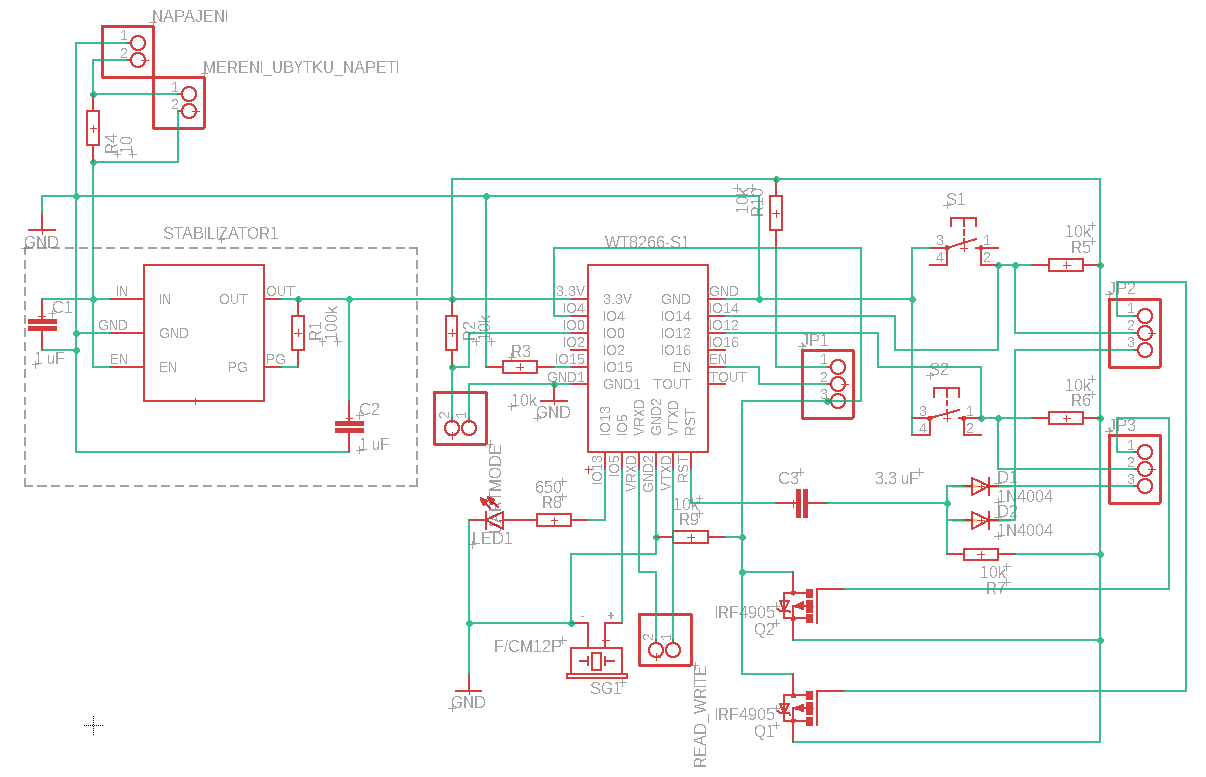
\includegraphics[width=12cm]{images/esp8266_schema}
        \caption{ESP8266 schéma zapojení}
        \label{fig:ESP8266_DPS}
    \end{figure}
    \subsubsection{Princip programu}
    Program nahraný v ESP8266 při zapnutí nejprve nastaví přídržný pin pro případ, že uživatel testuje enable button ustálený stav.
    Poté nastaví piny na čtení pro identifikaci správného zmáčknutého tlačítka pro sepnutí správné zásuvky.
    Program je ošetřen proti krátkému zmáčknutí tlačítek, kdy se ozve pípnutí bzučáku a rozsvícení LED\@.

    \section{Tvorba uživatelského rozhraní}
    Veškerý kód byl napsán v textovém editoru visual studio code s pluginem Platform.io, které usnadňuje některé metody používané v Arduino IDE.\\
    Cílem webové stránky je připojit ovladač do příslušné WiFi sítě, připojit až dvě zásuvky k ovladači a popřípadě upravit samotnou konfiguraci.

    \subsection{Nastavení webserveru}
    Pro možnost nastavení ESP jsem vybral metodu konfigurace přes webserver, kdy uživatel se připojí na IP adresu ESP pomocí svého internetového prohlížeče.
    ESP webserver se zapne pouze pokud uživatel vyžádá stisknutím obou interačních tlačítek najednou.
    Za podmínky, že ovladač není připojen k WiFi síti, vytvoří access point, kde je možné provést konfigura
    ci.
    Pokud je ovladač připojen k WiFi, může přistoupit k webové stránce pomocí IP adresy přidělenou přístupovým bodem.

    \subsection{Připojení k WiFi}
    Jakmile uživatel přistoupí na webovou stránku \viz{fig:website}, javascript požádá webserver o scannedWiFi.json.
    ESP poté naskenuje sítě, které se nachazí v okolí.
    Tyto sítě se uloží do pole tak, v jakém pořadí byly nalezeny.
    Pro zobrazení naskenovaných sítí na webových stránkách se vytvoří JSON string viz\ Uryvek kódu 1, který obsahuje počet naskenovaných sítí, pole s SSID\footnote{Identifikátor bezdrátové sítě WiFi}, pole s RSSI\footnote{Ukazatel síly signálu}, a pole, kde jsem označil zda se síť zabezpečena či nikoliv.
    RSSI jsem před zabalením do JSON pole přepočítal na sílu signálu v procentech.
    Po dokončení sestavení JSONu, odpoví na HTTP žádost javascriptu.
    Pomocí javascriptu a parametrů uložených v JSON zprávě se sestaví formuláře s jedním submit tlačítkem, které má na pozici value nastavené SSID.\\
    Pokud uživatel klikne na tlačítko s názvem dané WiFi sítě, je přesunut do adresa/wifi, kam uživatel zadá heslo.
    Heslo se odešle webserveru metodou POST, kde se autentizuje.
    Pokud síť není zabezpečena, začne probíhat připojení.

    \begin{figure}
        \centering
        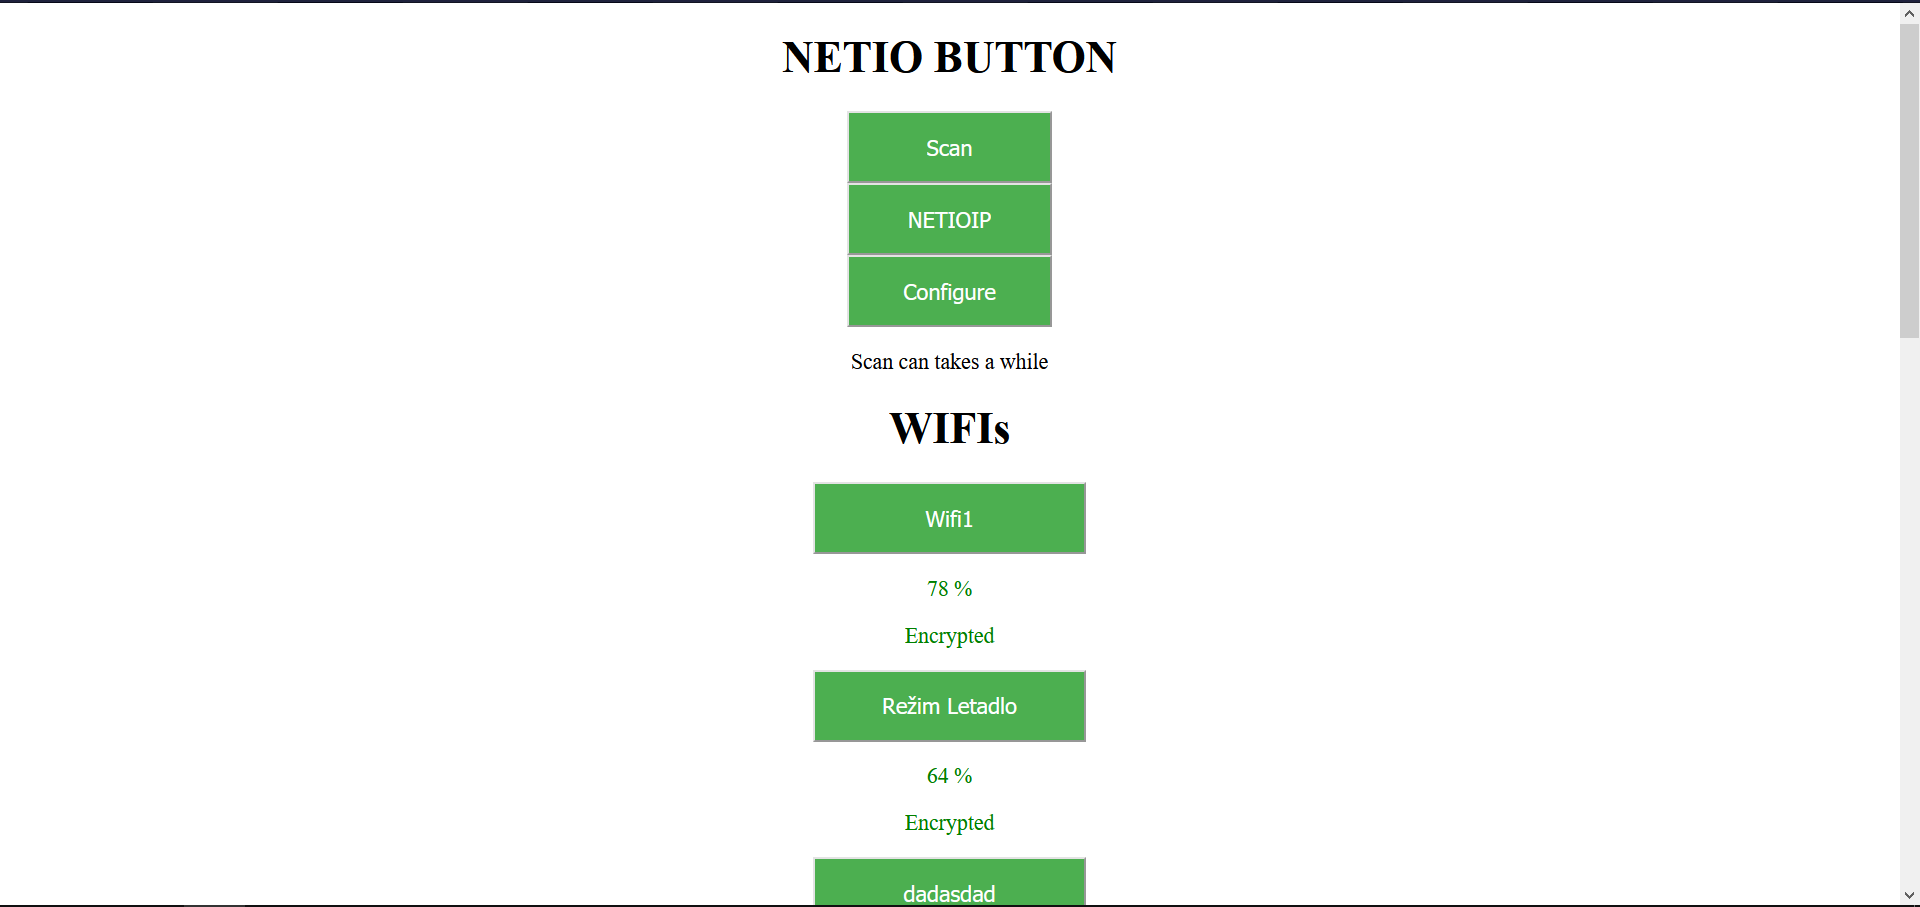
\includegraphics[width= 11cm]{images/webscreen}
        \caption{Webová stránka: výběr WiFi sítě}
        \label{fig:website}
    \end{figure}
    

    \subsection{Konfigurace reakce zásuvky}
    Pro komunikaci se zásuvkou ESP potřebuje znát IP adresu zásuvky a JSON zprávu, kterou bude odesílat.\\ Možnost konfigurace jsem uskutečnil pomocí HTML formulářů, který se metodou POST odesílá ESP. Aby ESP stále znalo uživatelskou konfiguraci i po restartu či spánku, musí si ji uložit.
    ESP dokáže uložit data do paměti pomocí knihovny EEPROM. Ve skutečnosti se nejedná o EEPROM paměť, která má velmi omezený počet zápisů a musí se vždy smazat celá paměť, ale ESP pouze emuluje EEPROM paměť.
    Ve skutečnosti tyto data ukládáme do FLASH paměti, což má řadu výhod.\\
    \begin{listing}[]
        \begin{minted}{cpp}
String jsonOfNetworks() {
    int numberOfNetworks = WiFi.scanNetworks();
    String networks = "{\"numOfNetworks\": \"";
    networks += numberOfNetworks;
    networks += "\", \"networks\": [";
    for (int i = 0; i < numberOfNetworks; i++) {
        networks += "\"";
        networks += WiFi.SSID(i);
        networks += "\"";
        networks += (i + 1 == numberOfNetworks) ? " " : ", ";
    }
    networks += "], \"strengh\": [";
    for (int i = 0; i < numberOfNetworks; i++) {
        networks += "\"";
        networks += dBmtoPercentage(WiFi.RSSI(i));
        networks += " %\" ";
        networks += (i + 1 == numberOfNetworks) ? " " : ", ";
    }
    networks += "], \"protection\": [";
    for (int i = 0; i < numberOfNetworks; i++) {
        networks += "\"";
        networks += (WiFi.encryptionType(i) == 0) ? "None" : "Encrypted";
        networks += "\" ";
        networks += (i + 1 == numberOfNetworks) ? " " : ", ";
    }
    networks += "]}";
    return networks;
}
        \end{minted}
        \label{lst:json}
        \caption{Tvorba JSON zprávy}
    \end{listing}
    Pro zápis do paměti jsem vytvořil funkci, která string rozdělí na jednotlivé charaktery a ty poté jednotlivě ukládá viz. Úryvek kódu 2.
    Jelikož velikost může být různá tak za poslední charakter se zapíše -1, což nastaví byte na 255 neboli nastaví ho na prázdný.
    Délky jsem nastavil pro IP adresy zásuvek na 15 charakterů a JSON zprávy na 100 charakterů.
    Načítání probíhá opačně.
    Načítá charaktery a složí je do stringu.
    Pokud narazí na byte 255, ukončí sestavení předčastně.\\
    Uživatel po dokončení nastavení ovladače ho může uspat.\\


    \begin{listing}[]
    \begin{minted}{cpp}
void saveToEEPROM(String sToSave, int startPosition) {
    char arr[sToSave.length() + 1];
    strcpy(arr, sToSave.c_str());
    for (int i = 0; i < sToSave.length(); i++) {
        EEPROM.write(startPosition + i, arr[i]);
    }
    EEPROM.write(startPosition + sToSave.length(), -1);
    EEPROM.commit();
    delay(500);
}

String readEEPROM(int numberOfStart, int len) {
    String tempString = "";
    for (int i = 0; i < len; i++) {
        char character = EEPROM.read(numberOfStart + i);
        if (character == 255)
            break;
        tempString += character;
    }
    return tempString;
}
    \end{minted}
    \label{listing:eeprom}
    \caption{Načítání a ukládání řetězců do/z paměti}
    \end{listing}



    \chapter{Závěr}
    \renewcommand\listoflistingscaption{Seznam úryvků kódu}
    \listoflistings
    \listoftables

    \listoffigures

    \prilohy{
        \kapitola{Příloha}
        \begin{figure}[h]
            \centering
            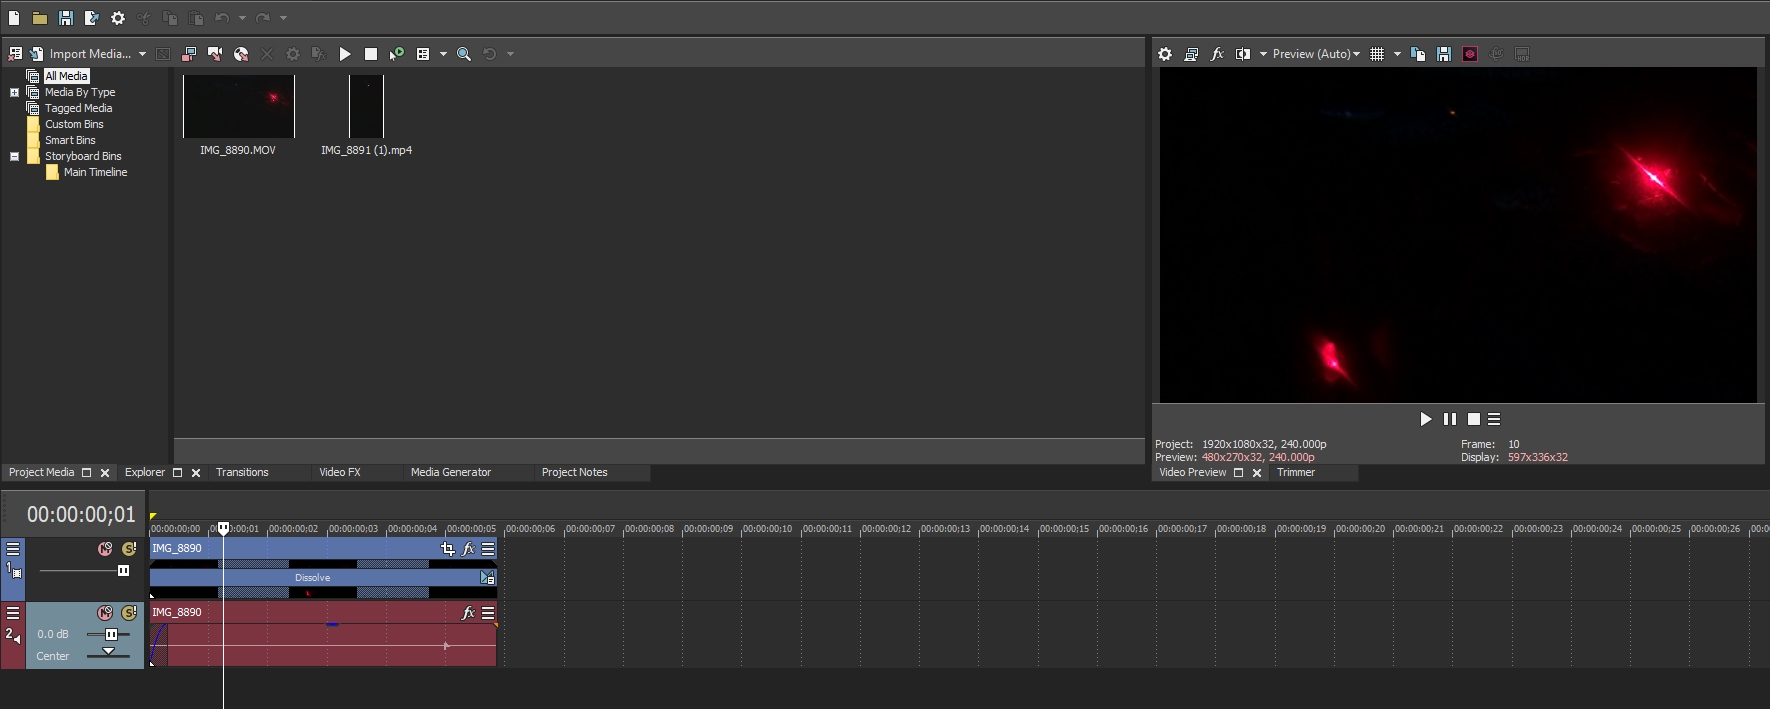
\includegraphics[width=12cm]{images/sonyvegaspostup}
            \caption{Ukázka postupu pro měření reakčních časů}
            \label{fig:sonyvegaspostup}
        \end{figure}
        \begin{figure}[h]
            \centering
            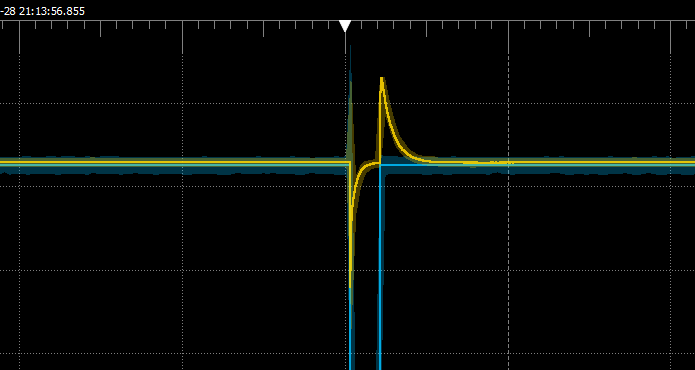
\includegraphics[width=12cm]{images/esp8266_3,3uf}
            \caption{ESP8266 reakce kondenzátoru graf}
            \label{fig:3.3uf-esp8266}
        \end{figure}
    }
    \bibliographystyle{czechiso}
    \bibliography{reference}

\end{document}
